\documentclass[12pt,]{book}
\usepackage{lmodern}
\usepackage{amssymb,amsmath}
\usepackage{ifxetex,ifluatex}
\usepackage{fixltx2e} % provides \textsubscript
\ifnum 0\ifxetex 1\fi\ifluatex 1\fi=0 % if pdftex
  \usepackage[T1]{fontenc}
  \usepackage[utf8]{inputenc}
\else % if luatex or xelatex
  \ifxetex
    \usepackage{mathspec}
  \else
    \usepackage{fontspec}
  \fi
  \defaultfontfeatures{Ligatures=TeX,Scale=MatchLowercase}
\fi
% use upquote if available, for straight quotes in verbatim environments
\IfFileExists{upquote.sty}{\usepackage{upquote}}{}
% use microtype if available
\IfFileExists{microtype.sty}{%
\usepackage{microtype}
\UseMicrotypeSet[protrusion]{basicmath} % disable protrusion for tt fonts
}{}
\usepackage{hyperref}
\hypersetup{unicode=true,
            pdftitle={금융 데이터 사이언스},
            pdfauthor={이현열},
            pdfborder={0 0 0},
            breaklinks=true}
\urlstyle{same}  % don't use monospace font for urls
\usepackage{natbib}
\bibliographystyle{apalike}
\usepackage{color}
\usepackage{fancyvrb}
\newcommand{\VerbBar}{|}
\newcommand{\VERB}{\Verb[commandchars=\\\{\}]}
\DefineVerbatimEnvironment{Highlighting}{Verbatim}{commandchars=\\\{\}}
% Add ',fontsize=\small' for more characters per line
\usepackage{framed}
\definecolor{shadecolor}{RGB}{248,248,248}
\newenvironment{Shaded}{\begin{snugshade}}{\end{snugshade}}
\newcommand{\AlertTok}[1]{\textcolor[rgb]{0.94,0.16,0.16}{#1}}
\newcommand{\AnnotationTok}[1]{\textcolor[rgb]{0.56,0.35,0.01}{\textbf{\textit{#1}}}}
\newcommand{\AttributeTok}[1]{\textcolor[rgb]{0.77,0.63,0.00}{#1}}
\newcommand{\BaseNTok}[1]{\textcolor[rgb]{0.00,0.00,0.81}{#1}}
\newcommand{\BuiltInTok}[1]{#1}
\newcommand{\CharTok}[1]{\textcolor[rgb]{0.31,0.60,0.02}{#1}}
\newcommand{\CommentTok}[1]{\textcolor[rgb]{0.56,0.35,0.01}{\textit{#1}}}
\newcommand{\CommentVarTok}[1]{\textcolor[rgb]{0.56,0.35,0.01}{\textbf{\textit{#1}}}}
\newcommand{\ConstantTok}[1]{\textcolor[rgb]{0.00,0.00,0.00}{#1}}
\newcommand{\ControlFlowTok}[1]{\textcolor[rgb]{0.13,0.29,0.53}{\textbf{#1}}}
\newcommand{\DataTypeTok}[1]{\textcolor[rgb]{0.13,0.29,0.53}{#1}}
\newcommand{\DecValTok}[1]{\textcolor[rgb]{0.00,0.00,0.81}{#1}}
\newcommand{\DocumentationTok}[1]{\textcolor[rgb]{0.56,0.35,0.01}{\textbf{\textit{#1}}}}
\newcommand{\ErrorTok}[1]{\textcolor[rgb]{0.64,0.00,0.00}{\textbf{#1}}}
\newcommand{\ExtensionTok}[1]{#1}
\newcommand{\FloatTok}[1]{\textcolor[rgb]{0.00,0.00,0.81}{#1}}
\newcommand{\FunctionTok}[1]{\textcolor[rgb]{0.00,0.00,0.00}{#1}}
\newcommand{\ImportTok}[1]{#1}
\newcommand{\InformationTok}[1]{\textcolor[rgb]{0.56,0.35,0.01}{\textbf{\textit{#1}}}}
\newcommand{\KeywordTok}[1]{\textcolor[rgb]{0.13,0.29,0.53}{\textbf{#1}}}
\newcommand{\NormalTok}[1]{#1}
\newcommand{\OperatorTok}[1]{\textcolor[rgb]{0.81,0.36,0.00}{\textbf{#1}}}
\newcommand{\OtherTok}[1]{\textcolor[rgb]{0.56,0.35,0.01}{#1}}
\newcommand{\PreprocessorTok}[1]{\textcolor[rgb]{0.56,0.35,0.01}{\textit{#1}}}
\newcommand{\RegionMarkerTok}[1]{#1}
\newcommand{\SpecialCharTok}[1]{\textcolor[rgb]{0.00,0.00,0.00}{#1}}
\newcommand{\SpecialStringTok}[1]{\textcolor[rgb]{0.31,0.60,0.02}{#1}}
\newcommand{\StringTok}[1]{\textcolor[rgb]{0.31,0.60,0.02}{#1}}
\newcommand{\VariableTok}[1]{\textcolor[rgb]{0.00,0.00,0.00}{#1}}
\newcommand{\VerbatimStringTok}[1]{\textcolor[rgb]{0.31,0.60,0.02}{#1}}
\newcommand{\WarningTok}[1]{\textcolor[rgb]{0.56,0.35,0.01}{\textbf{\textit{#1}}}}
\usepackage{longtable,booktabs}
\usepackage{graphicx}
% grffile has become a legacy package: https://ctan.org/pkg/grffile
\IfFileExists{grffile.sty}{%
\usepackage{grffile}
}{}
\makeatletter
\def\maxwidth{\ifdim\Gin@nat@width>\linewidth\linewidth\else\Gin@nat@width\fi}
\def\maxheight{\ifdim\Gin@nat@height>\textheight\textheight\else\Gin@nat@height\fi}
\makeatother
% Scale images if necessary, so that they will not overflow the page
% margins by default, and it is still possible to overwrite the defaults
% using explicit options in \includegraphics[width, height, ...]{}
\setkeys{Gin}{width=\maxwidth,height=\maxheight,keepaspectratio}
\IfFileExists{parskip.sty}{%
\usepackage{parskip}
}{% else
\setlength{\parindent}{0pt}
\setlength{\parskip}{6pt plus 2pt minus 1pt}
}
\setlength{\emergencystretch}{3em}  % prevent overfull lines
\providecommand{\tightlist}{%
  \setlength{\itemsep}{0pt}\setlength{\parskip}{0pt}}
\setcounter{secnumdepth}{5}
% Redefines (sub)paragraphs to behave more like sections
\ifx\paragraph\undefined\else
\let\oldparagraph\paragraph
\renewcommand{\paragraph}[1]{\oldparagraph{#1}\mbox{}}
\fi
\ifx\subparagraph\undefined\else
\let\oldsubparagraph\subparagraph
\renewcommand{\subparagraph}[1]{\oldsubparagraph{#1}\mbox{}}
\fi

%%% Use protect on footnotes to avoid problems with footnotes in titles
\let\rmarkdownfootnote\footnote%
\def\footnote{\protect\rmarkdownfootnote}

%%% Change title format to be more compact
\usepackage{titling}

% Create subtitle command for use in maketitle
\providecommand{\subtitle}[1]{
  \posttitle{
    \begin{center}\large#1\end{center}
    }
}

\setlength{\droptitle}{-2em}

  \title{금융 데이터 사이언스}
    \pretitle{\vspace{\droptitle}\centering\huge}
  \posttitle{\par}
    \author{이현열}
    \preauthor{\centering\large\emph}
  \postauthor{\par}
      \predate{\centering\large\emph}
  \postdate{\par}
    \date{2019-11-19}

\usepackage{kotex}
\usepackage{booktabs}
\usepackage{amsthm}
\usepackage{float}
\usepackage[paperwidth=6.9in, paperheight=9.8in, margin=2cm]{geometry}
\usepackage[Sonny]{fncychap} 
\makeatletter
\def\thm@space@setup{%
  \thm@preskip=8pt plus 2pt minus 4pt
  \thm@postskip=\thm@preskip
}
\makeatother
\usepackage{booktabs}
\usepackage{longtable}
\usepackage{array}
\usepackage{multirow}
\usepackage{wrapfig}
\usepackage{float}
\usepackage{colortbl}
\usepackage{pdflscape}
\usepackage{tabu}
\usepackage{threeparttable}
\usepackage{threeparttablex}
\usepackage[normalem]{ulem}
\usepackage{makecell}
\usepackage{xcolor}

\begin{document}
\maketitle

{
\setcounter{tocdepth}{1}
\tableofcontents
}
\hypertarget{welcome}{%
\chapter*{Welcome}\label{welcome}}
\addcontentsline{toc}{chapter}{Welcome}

R을 이용한 금융 데이터 사이언스 과정 페이지 입니다.
현재 머신러닝 파트만 업로드 중입니다.

\hypertarget{uxba38uxc2e0uxb7ecuxb2dduxc774uxb780}{%
\chapter{머신러닝이란?}\label{uxba38uxc2e0uxb7ecuxb2dduxc774uxb780}}

머신러닝이란 데이터에서 패턴을 찾아 새로운 데이터의 결과값을 예측하는 방법이며 크게 지도학습, 비지도학습, 강화학습으로 나눌수 있습니다.

\hypertarget{uxc9c0uxb3c4uxd559uxc2b5supervised-learning}{%
\section{지도학습(Supervised Learning)}\label{uxc9c0uxb3c4uxd559uxc2b5supervised-learning}}

지도학습은 정답을 알려주며 학습시키는 것입니다. 예를들어 고양이 사진을 준 후(input data), 이 사진은 고양이(label data)라는 것를 알려준 후, 이러한 패턴을 바탕으로 새로운 데이터의 결과값을 예측하는 방식입니다. 따라서 기계가 정답을 잘 맞췄는지 아닌지 쉽게 알 수 있다. 지도학습에는 크게 분류(classification)과 회귀(regression)가 있습니다.

\begin{itemize}
\item
  분류(classification): 두 가지 혹은 여러 값 중 하나로 분류하는 것입니다. 예를 들어 특정 이메일이 스팸인가 아닌가 혹은 개인의 신용등급을 분류하는 방식입니다.
\item
  회귀(regression): 어떤 데이터들의 특징(feature)을 토대로 값을 예측하는 것입니다.
\end{itemize}

\hypertarget{uxbe44uxc9c0uxb3c4uxd559uxc2b5unsupervised-learning}{%
\section{비지도학습(Unsupervised Learning)}\label{uxbe44uxc9c0uxb3c4uxd559uxc2b5unsupervised-learning}}

정답(label)을 따로 알려주지 않은 상태에서, 비슷한 데이터들을 군집화 하는 것입니다.

예를들어 고양이, 병아리, 기린, 호랑이 사진을 비지도학습 시킬 경우, 각 사진이 무슨 동물인지 정답(label)을 알려주지 않았기 때문에 이 동물이 '무엇'이라고 기계가 정의는 할 수 없지만 비슷한 단위로 군집화 해준다.다리가 4개인 고양이와 호랑이를 한 분류로 묶고, 다리가 4개지만 목이 긴 기린은 다른 분류로, 다리가 얇고 몸통이 둥그런 병아리는 또 다른 분류로 나누어 놓을 것입니다.

\begin{center}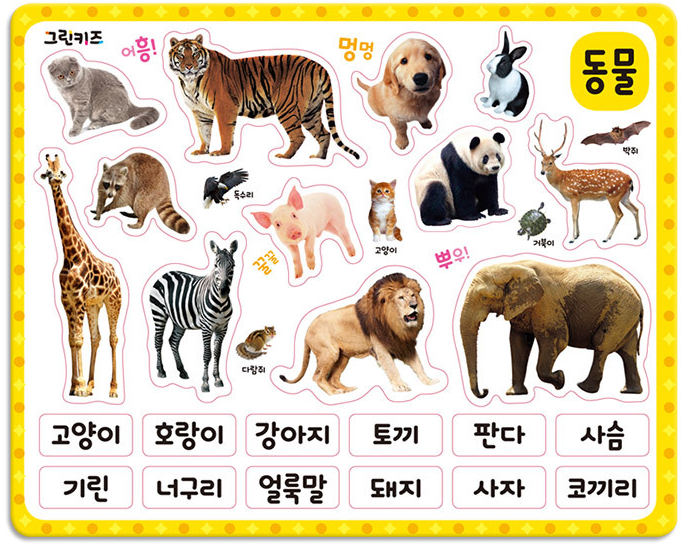
\includegraphics[width=0.5\linewidth]{images/animal} \end{center}

실무에서는 지도학습에서의 적절한 feature를 찾아내기 위한 전처리 방법으로 비지도 학습을 쓰기도 합니다.

\hypertarget{uxb525uxb7ecuxb2dd-uxac15uxd654uxd559uxc2b5reinforcement-learning}{%
\section{딥러닝 / 강화학습(Reinforcement Learning)}\label{uxb525uxb7ecuxb2dd-uxac15uxd654uxd559uxc2b5reinforcement-learning}}

상과 벌이라는 보상(reward)을 주며 상을 최대화하고 벌을 최소화 하도록 강화 학습하는 방식입니다. 알파고가 이 방법으로 학습 되었고, 주로 게임에서 최적의 동작을 찾는데 쓰는 학습 방식입니다.

\hypertarget{uxc0acuxc6a9-uxd328uxd0a4uxc9c0}{%
\section{사용 패키지}\label{uxc0acuxc6a9-uxd328uxd0a4uxc9c0}}

본 과정에서 사용되는 패키지는 다음과 같이 설치할 수 있습니다. (업데이트 중)

\begin{Shaded}
\begin{Highlighting}[]
\NormalTok{pkg =}\StringTok{ }\KeywordTok{c}\NormalTok{(}\StringTok{'alr3'}\NormalTok{, }\StringTok{'caret'}\NormalTok{, }\StringTok{'ISLR'}\NormalTok{, }\StringTok{'MASS'}\NormalTok{, }\StringTok{'InformationValue'}\NormalTok{,}
        \StringTok{'leaps'}\NormalTok{, }\StringTok{'car'}\NormalTok{, }\StringTok{'corrplot'}\NormalTok{, }\StringTok{'lmtest'}\NormalTok{, }\StringTok{'bestglm'}\NormalTok{,}
        \StringTok{'ElemStatLearn'}\NormalTok{)}

\NormalTok{new.pkg =}\StringTok{ }\NormalTok{pkg[}\OperatorTok{!}\NormalTok{(pkg }\OperatorTok\StringTok{ }\KeywordTok{installed.packages}\NormalTok{()[, }\StringTok{"Package"}\NormalTok{])]}
\ControlFlowTok{if}\NormalTok{ (}\KeywordTok{length}\NormalTok{(new.pkg)) \{}
  \KeywordTok{install.packages}\NormalTok{(new.pkg, }\DataTypeTok{dependencies =} \OtherTok{TRUE}\NormalTok{)\}}
\end{Highlighting}
\end{Shaded}

\hypertarget{uxd68cuxadc0uxbd84uxc11d}{%
\chapter{회귀분석}\label{uxd68cuxadc0uxbd84uxc11d}}

\hypertarget{uxc0c1uxad00uxad00uxacc4-uxc774uxd574uxd558uxae30}{%
\section{상관관계 이해하기}\label{uxc0c1uxad00uxad00uxacc4-uxc774uxd574uxd558uxae30}}

먼저 R에서 제공하는 기본 데이터를 불러옵니다.

\begin{Shaded}
\begin{Highlighting}[]
\KeywordTok{data}\NormalTok{(anscombe)}
\KeywordTok{attach}\NormalTok{(anscombe)}
\KeywordTok{head}\NormalTok{(anscombe)}
\end{Highlighting}
\end{Shaded}

\begin{verbatim}
##   x1 x2 x3 x4   y1   y2    y3   y4
## 1 10 10 10  8 8.04 9.14  7.46 6.58
## 2  8  8  8  8 6.95 8.14  6.77 5.76
## 3 13 13 13  8 7.58 8.74 12.74 7.71
## 4  9  9  9  8 8.81 8.77  7.11 8.84
## 5 11 11 11  8 8.33 9.26  7.81 8.47
## 6 14 14 14  8 9.96 8.10  8.84 7.04
\end{verbatim}

각 변수의 상관관계를 살펴보도록 합니다.

\begin{Shaded}
\begin{Highlighting}[]
\KeywordTok{cor}\NormalTok{(x1, y1)}
\end{Highlighting}
\end{Shaded}

\begin{verbatim}
## [1] 0.8164
\end{verbatim}

\begin{Shaded}
\begin{Highlighting}[]
\KeywordTok{cor}\NormalTok{(x2, y2)}
\end{Highlighting}
\end{Shaded}

\begin{verbatim}
## [1] 0.8162
\end{verbatim}

둘 간의 상관관계는 0.8164로 동일합니다. 이를 그림으로 확인해보도록 합니다.

\begin{Shaded}
\begin{Highlighting}[]
\KeywordTok{par}\NormalTok{(}\DataTypeTok{mfrow =} \KeywordTok{c}\NormalTok{(}\DecValTok{2}\NormalTok{, }\DecValTok{2}\NormalTok{))}
\KeywordTok{plot}\NormalTok{(x1, y1, }\DataTypeTok{main =} \StringTok{'Plot 1'}\NormalTok{)}
\KeywordTok{plot}\NormalTok{(x2, y2, }\DataTypeTok{main =} \StringTok{'Plot 2'}\NormalTok{)}
\KeywordTok{plot}\NormalTok{(x3, y3, }\DataTypeTok{main =} \StringTok{'Plot 3'}\NormalTok{)}
\KeywordTok{plot}\NormalTok{(x4, y4, }\DataTypeTok{main =} \StringTok{'Plot 4'}\NormalTok{)}
\end{Highlighting}
\end{Shaded}

\begin{center}\includegraphics[width=0.5\linewidth]{02-regression_files/figure-latex/unnamed-chunk-4-1} \end{center}

Plot 1은 선형관계를, Plot 2는 곡선 모양을, Plot 3은 특이점이, Plot 4는 특이점 하나만이 상관관계가 있는것 처럼 보입니다. 이처럼 상관관계에만 전적으로 의존하면 제대로 된 결과를 확인할 수 없습니다.

\hypertarget{uxd68cuxadc0uxc758-uxc774uxd574}{%
\section{회귀의 이해}\label{uxd68cuxadc0uxc758-uxc774uxd574}}

회귀분석의 식은 다음과 같이 나타납니다.

\(y = a + bx\)

\begin{itemize}
\tightlist
\item
  \(y\): 종속변수
\item
  \(x\): 독립변수
\item
  \(b\): 기울기. \(x\)가 증가할 때마다 직선이 얼마나 올라가는지를 명시
\item
  \(a\): 절편. 직선이 세로 \(y\)축과 교차하는 지점을 명시
\end{itemize}

\hypertarget{uxbcf4uxd1b5-uxcd5cuxc18c-uxc81cuxacf1ols-uxcd94uxc815}{%
\subsection{보통 최소 제곱(OLS) 추정}\label{uxbcf4uxd1b5-uxcd5cuxc18c-uxc81cuxacf1ols-uxcd94uxc815}}

OLS 회귀의 목표는 다음 방정식을 최소화하는 작업입니다.

\begin{itemize}
\tightlist
\item
  \(\sum(y_i - \hat{y_i})^2 = \sum{e_i}^2\)
\end{itemize}

즉 실제 값과 예측 값의 차로 \(e\)(오차)를 정의됩니다.

\(\bar{y} = a + b\bar{x}\)에서 다음식이 유도됩니다.

\begin{itemize}
\tightlist
\item
  \(a = \bar{y} - b\bar{x}\)
\item
  \(b = \frac{\sum(x_i - \bar{x})(y_i - \bar{y})}{\sum(x_i - \bar{x})^2}\)
\item
  \(Var(x) = \frac{\sum(x_i - \bar{x})^2}{n}\)
\item
  \(Cov(x,y) = \frac{\sum(x_i - \bar{x})(y_i - \bar{y})}{n}\)
\end{itemize}

따라서 b는 다음과 같이 나타낼 수 있습니다.

\begin{itemize}
\tightlist
\item
  \(b = \frac{Cov(x,y)}{Var(x)}\)
\end{itemize}

R에서 해당 계수는 \texttt{lm()} 함수를 이용해 손쉽게 추정할 수 있습니다.

\hypertarget{uxb2e8uxbcc0uxb7c9-uxd68cuxadc0uxbd84uxc11d}{%
\section{단변량 회귀분석}\label{uxb2e8uxbcc0uxb7c9-uxd68cuxadc0uxbd84uxc11d}}

\hypertarget{uxcc4cuxb9b0uxc800-uxd638-uxb370uxc774uxd130}{%
\subsection{챌린저 호 데이터}\label{uxcc4cuxb9b0uxc800-uxd638-uxb370uxc774uxd130}}

미국 우주왕복선 챌린저가 로켓 부스터 고장으로 분해되면서 일곱 명의 승무원이 사망했으며, 잠재 요인으로 발사 온도가 의심되었습니다. 로켓 연결 부분의 밀봉을 담당하는 패킹용 고무 오링이 40°F 미만에서는 테스트되지 않았었고, 발사일의 날씨가 평소와 달리 매우 춥고 영하(31°F)인 상태였기 때문입니다.

다음 데이터는 온도에 따른 오링의 손상여부 테스트 데이터입니다.

\begin{Shaded}
\begin{Highlighting}[]
\NormalTok{challenger =}\StringTok{ }\KeywordTok{read.csv}\NormalTok{(}\StringTok{'http://www.math.usu.edu/~symanzik/teaching/2009_stat6560/RDataAndScripts/sharif_abbass_project1_challenger.csv'}\NormalTok{)}

\KeywordTok{plot}\NormalTok{(challenger}\OperatorTok{$}\NormalTok{temperature, challenger}\OperatorTok{$}\NormalTok{r,}
     \DataTypeTok{xlab =} \StringTok{'Temp'}\NormalTok{, }\DataTypeTok{ylab =} \StringTok{'Damage'}\NormalTok{, }\DataTypeTok{pch =} \DecValTok{1}\NormalTok{)}
\KeywordTok{abline}\NormalTok{(}\DataTypeTok{v =} \DecValTok{65}\NormalTok{)}
\end{Highlighting}
\end{Shaded}

\begin{center}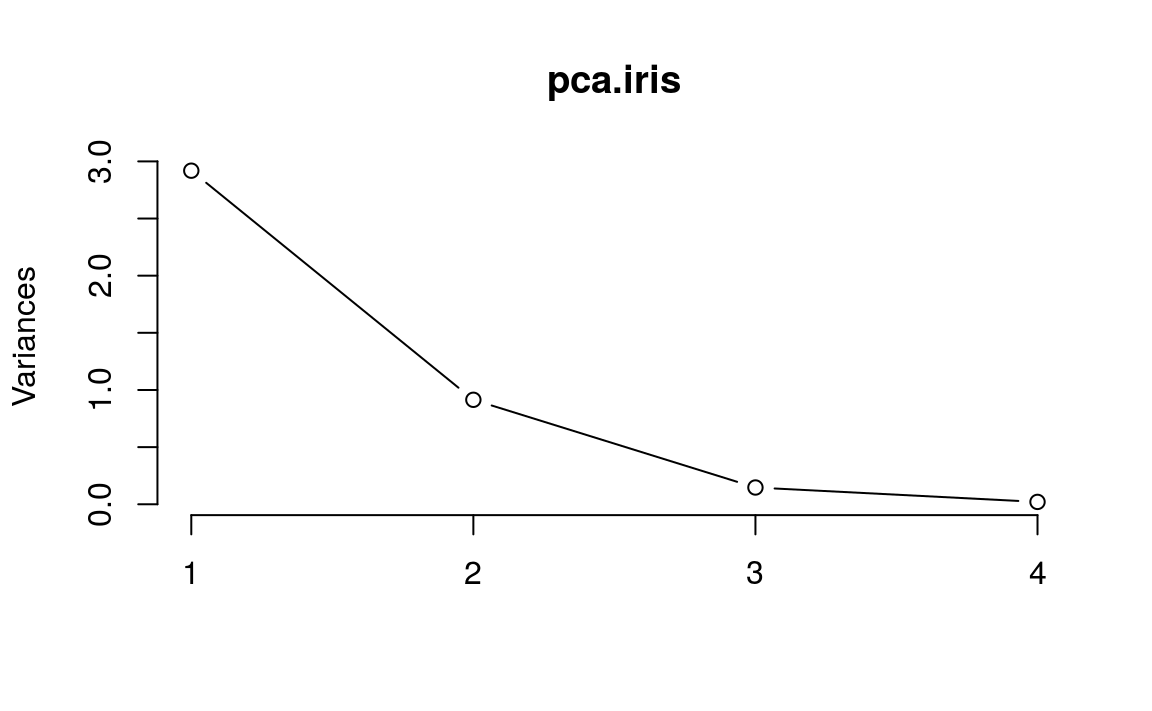
\includegraphics[width=0.5\linewidth]{02-regression_files/figure-latex/unnamed-chunk-5-1} \end{center}

고온에서 발사될 때 오링의 손상 이벤트가 적어지는 경향이 있습니다. 회귀분석을 통해 둘간의 관계를 살펴보도록 합니다.

\begin{Shaded}
\begin{Highlighting}[]
\NormalTok{reg.challenger=}\StringTok{ }\KeywordTok{lm}\NormalTok{(r }\OperatorTok{~}\StringTok{ }\NormalTok{temperature, }\DataTypeTok{data =}\NormalTok{ challenger)}
\KeywordTok{summary}\NormalTok{(reg.challenger)}
\end{Highlighting}
\end{Shaded}

\begin{verbatim}
## 
## Call:
## lm(formula = r ~ temperature, data = challenger)
## 
## Residuals:
##     Min      1Q  Median      3Q     Max 
## -0.5608 -0.3944 -0.0854  0.1056  1.8671 
## 
## Coefficients:
##             Estimate Std. Error t value Pr(>|t|)   
## (Intercept)   3.6984     1.2195    3.03   0.0063 **
## temperature  -0.0475     0.0174   -2.73   0.0127 * 
## ---
## Signif. codes:  
## 0 '***' 0.001 '**' 0.01 '*' 0.05 '.' 0.1 ' ' 1
## 
## Residual standard error: 0.577 on 21 degrees of freedom
## Multiple R-squared:  0.261,  Adjusted R-squared:  0.226 
## F-statistic: 7.43 on 1 and 21 DF,  p-value: 0.0127
\end{verbatim}

temperature의 회귀계수가 -0.05로써 온도와 손상 이벤트 간에는 역의 관계가 있음이 보입니다. 당시 온도인 31°F를 대입하면 오링의 예상 손상 이벤트는 \(3.69841 + 31 \times (-0.04754) = 2.22467\) 이 됩니다.

회귀분석 결과를 그림으로 확인해보도록 하겠습니다.

\begin{Shaded}
\begin{Highlighting}[]
\KeywordTok{plot}\NormalTok{(challenger}\OperatorTok{$}\NormalTok{temperature, challenger}\OperatorTok{$}\NormalTok{r,}
     \DataTypeTok{xlab =} \StringTok{'Temp'}\NormalTok{, }\DataTypeTok{ylab =} \StringTok{'Damage'}\NormalTok{, }\DataTypeTok{pch =} \DecValTok{1}\NormalTok{)}
\KeywordTok{abline}\NormalTok{(reg.challenger, }\DataTypeTok{lwd =} \DecValTok{3}\NormalTok{, }\DataTypeTok{col =} \StringTok{'red'}\NormalTok{)}
\end{Highlighting}
\end{Shaded}

\begin{center}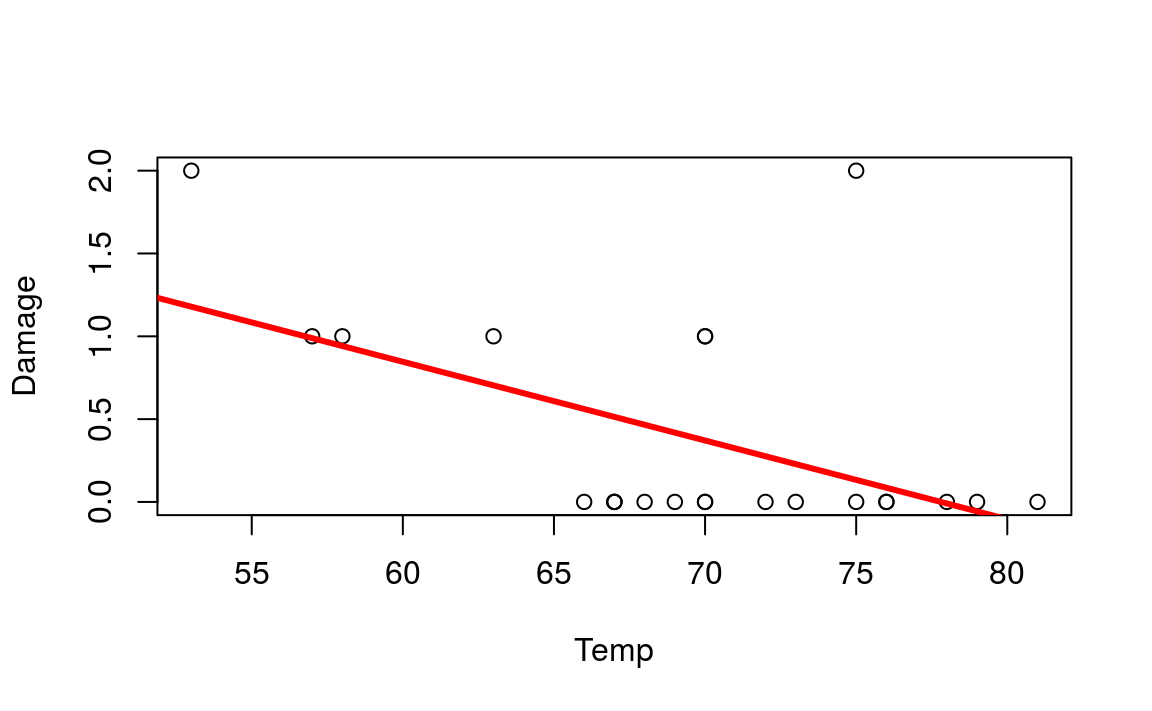
\includegraphics[width=0.5\linewidth]{02-regression_files/figure-latex/unnamed-chunk-7-1} \end{center}

\hypertarget{uxbbf8uxad6d-uxc640uxc774uxc624uxbc0d-uxc8fc-uxc6a9uxcd9cuxb7c9-uxc608uxce21}{%
\subsection{미국 와이오밍 주 용출량 예측}\label{uxbbf8uxad6d-uxc640uxc774uxc624uxbc0d-uxc8fc-uxc6a9uxcd9cuxb7c9-uxc608uxce21}}

미국 와이오밍 주 스네이크 강 유역의 용출량을 예측변수, 해당 연도 눈의 강우량을 이용하여 예측합니다. 먼저 해당 데이터를 그림으로 나타내봅니다.

\begin{Shaded}
\begin{Highlighting}[]
\KeywordTok{library}\NormalTok{(alr3)}
\KeywordTok{data}\NormalTok{(snake)}
\KeywordTok{colnames}\NormalTok{(snake) =}\StringTok{ }\KeywordTok{c}\NormalTok{(}\StringTok{'content'}\NormalTok{, }\StringTok{'yield'}\NormalTok{)}
\KeywordTok{head}\NormalTok{(snake)}
\end{Highlighting}
\end{Shaded}

\begin{verbatim}
##   content yield
## 1    23.1  10.5
## 2    32.8  16.7
## 3    31.8  18.2
## 4    32.0  17.0
## 5    30.4  16.3
## 6    24.0  10.5
\end{verbatim}

\begin{Shaded}
\begin{Highlighting}[]
\KeywordTok{plot}\NormalTok{(snake, }\DataTypeTok{xlab =} \StringTok{'water content of snow'}\NormalTok{,}
     \DataTypeTok{ylab =} \StringTok{'water yield'}\NormalTok{)}
\end{Highlighting}
\end{Shaded}

\begin{center}\includegraphics[width=0.5\linewidth]{02-regression_files/figure-latex/unnamed-chunk-8-1} \end{center}

양 끝에 특이점 두개가 있습니다. 다음으로 \texttt{lm()} 함수를 이용해 단변량 회귀분석을 실행합니다.

\begin{Shaded}
\begin{Highlighting}[]
\NormalTok{reg =}\StringTok{ }\KeywordTok{lm}\NormalTok{(yield }\OperatorTok{~}\StringTok{ }\NormalTok{content, }\DataTypeTok{data =}\NormalTok{ snake)}
\KeywordTok{summary}\NormalTok{(reg)}
\end{Highlighting}
\end{Shaded}

\begin{verbatim}
## 
## Call:
## lm(formula = yield ~ content, data = snake)
## 
## Residuals:
##    Min     1Q Median     3Q    Max 
## -2.179 -1.515 -0.362  1.628  3.197 
## 
## Coefficients:
##             Estimate Std. Error t value    Pr(>|t|)    
## (Intercept)   0.7254     1.5488    0.47        0.65    
## content       0.4981     0.0495   10.06 0.000000046 ***
## ---
## Signif. codes:  
## 0 '***' 0.001 '**' 0.01 '*' 0.05 '.' 0.1 ' ' 1
## 
## Residual standard error: 1.74 on 15 degrees of freedom
## Multiple R-squared:  0.871,  Adjusted R-squared:  0.862 
## F-statistic:  101 on 1 and 15 DF,  p-value: 0.0000000463
\end{verbatim}

content 변수가 유의미한 변수임이 확인됩니다. 다음으로 산포도에 회귀식을 그려보도록 하겠습니다.

\begin{Shaded}
\begin{Highlighting}[]
\KeywordTok{plot}\NormalTok{(snake, }\DataTypeTok{xlab =} \StringTok{'water content of snow'}\NormalTok{,}
     \DataTypeTok{ylab =} \StringTok{'water yield'}\NormalTok{)}
\KeywordTok{abline}\NormalTok{(reg, }\DataTypeTok{lwd =} \DecValTok{3}\NormalTok{, }\DataTypeTok{col =} \StringTok{'red'}\NormalTok{)}
\end{Highlighting}
\end{Shaded}

\begin{center}\includegraphics[width=0.5\linewidth]{02-regression_files/figure-latex/unnamed-chunk-10-1} \end{center}

회귀분석의 가정은 다음과 같습니다.

\begin{itemize}
\tightlist
\item
  선형성(linearity): 독립 변수(x)와 종속 변수(y) 사이에 선형적 관계
\item
  오류항의 비상관(non-correlation): 오류항 사이에 상관관계가 없음
\item
  등분산성(homoscedasticity): 오류항은 정규분포를 따르며 일정한 분산을 가짐. 이 가정을 위배되면 이분산성(heteroscedasticity)
\item
  비공선성(non-collinearity): 두 예측 변수 사이에도 선형적인 관계가 있으면 안됨
\item
  특이점의 부재(absence of outliers): 특이점이 있으면 추정값이 심하게 왜곡될 수 있음
\end{itemize}

회귀분석 결과에 \texttt{plot()} 함수를 입력하여 해당 가정을 확인할 수 있습니다.

\begin{Shaded}
\begin{Highlighting}[]
\KeywordTok{par}\NormalTok{(}\DataTypeTok{mfrow =} \KeywordTok{c}\NormalTok{(}\DecValTok{2}\NormalTok{, }\DecValTok{2}\NormalTok{))}
\KeywordTok{plot}\NormalTok{(reg)}
\end{Highlighting}
\end{Shaded}

\begin{center}
\includegraphics[width=0.5\linewidth]{02-regression_files/figure-latex/unnamed-chunk-11-1} \end{center}

car 패키지의 \texttt{qqPlot()} 함수를 통해 Q-Q 플롯의 신뢰구간을 확인할 수 있습니다.

\begin{Shaded}
\begin{Highlighting}[]
\KeywordTok{qqPlot}\NormalTok{(reg)}
\end{Highlighting}
\end{Shaded}

\begin{verbatim}
## [1]  7 10
\end{verbatim}

\begin{center}\includegraphics[width=0.5\linewidth]{02-regression_files/figure-latex/unnamed-chunk-12-1} \end{center}

\hypertarget{uxb2e4uxbcc0uxb7c9-uxd68cuxadc0uxbd84uxc11d}{%
\section{다변량 회귀분석}\label{uxb2e4uxbcc0uxb7c9-uxd68cuxadc0uxbd84uxc11d}}

\hypertarget{uxb2e4uxc774uxc544uxbaacuxb4dc-uxb370uxc774uxd130}{%
\subsection{다이아몬드 데이터}\label{uxb2e4uxc774uxc544uxbaacuxb4dc-uxb370uxc774uxd130}}

다이아몬드 가격에 영향을 미치는 요소에 대해 회귀분석을 실시하도록 합니다.

\begin{Shaded}
\begin{Highlighting}[]
\KeywordTok{library}\NormalTok{(caret)}

\KeywordTok{data}\NormalTok{(diamonds)}
\KeywordTok{head}\NormalTok{(diamonds)}
\end{Highlighting}
\end{Shaded}

\begin{verbatim}
## # A tibble: 6 x 10
##   carat cut   color clarity depth table price     x
##   <dbl> <ord> <ord> <ord>   <dbl> <dbl> <int> <dbl>
## 1 0.23  Ideal E     SI2      61.5    55   326  3.95
## 2 0.21  Prem~ E     SI1      59.8    61   326  3.89
## 3 0.23  Good  E     VS1      56.9    65   327  4.05
## 4 0.290 Prem~ I     VS2      62.4    58   334  4.2 
## 5 0.31  Good  J     SI2      63.3    58   335  4.34
## 6 0.24  Very~ J     VVS2     62.8    57   336  3.94
## # ... with 2 more variables: y <dbl>, z <dbl>
\end{verbatim}

종속변수로 price, 독립변수로 caret, depth, table 피처를 사용하도록 하겠습니다.

\begin{itemize}
\tightlist
\item
  caret: 다이아몬드 무게
\item
  depth: 깊이 비율, z / mean(x, y)
\item
  table: 가장 넓은 부분의 너비 대비 다이아몬드 꼭대기의 너비
\end{itemize}

\begin{Shaded}
\begin{Highlighting}[]
\NormalTok{reg.diamonds =}\StringTok{ }\KeywordTok{lm}\NormalTok{(price }\OperatorTok{~}\StringTok{ }\NormalTok{carat }\OperatorTok{+}\StringTok{ }\NormalTok{depth }\OperatorTok{+}\StringTok{ }\NormalTok{table, }\DataTypeTok{data =}\NormalTok{ diamonds)}
\KeywordTok{summary}\NormalTok{(reg.diamonds)}
\end{Highlighting}
\end{Shaded}

\begin{verbatim}
## 
## Call:
## lm(formula = price ~ carat + depth + table, data = diamonds)
## 
## Residuals:
##    Min     1Q Median     3Q    Max 
## -18288   -786    -33    527  12487 
## 
## Coefficients:
##             Estimate Std. Error t value Pr(>|t|)    
## (Intercept) 13003.44     390.92    33.3   <2e-16 ***
## carat        7858.77      14.15   555.4   <2e-16 ***
## depth        -151.24       4.82   -31.4   <2e-16 ***
## table        -104.47       3.14   -33.3   <2e-16 ***
## ---
## Signif. codes:  
## 0 '***' 0.001 '**' 0.01 '*' 0.05 '.' 0.1 ' ' 1
## 
## Residual standard error: 1530 on 53936 degrees of freedom
## Multiple R-squared:  0.854,  Adjusted R-squared:  0.854 
## F-statistic: 1.05e+05 on 3 and 53936 DF,  p-value: <2e-16
\end{verbatim}

price와 carat은 양의 관계, depth와 table은 음의 관계가 있습니다.

\hypertarget{uxce98uxb9acuxd3ecuxb2c8uxc544-uxbb3c-uxac00uxc6a9uxb7c9}{%
\subsection{캘리포니아 물 가용량}\label{uxce98uxb9acuxd3ecuxb2c8uxc544-uxbb3c-uxac00uxc6a9uxb7c9}}

캘리포니아 오웬스 벨리의 여섯 지점에서 측정한 강설량을 토대로 물 가용량을 예측해보도록 하겠습니다.

\begin{Shaded}
\begin{Highlighting}[]
\KeywordTok{data}\NormalTok{(water)}
\KeywordTok{str}\NormalTok{(water)}
\end{Highlighting}
\end{Shaded}

\begin{verbatim}
## 'data.frame':    43 obs. of  8 variables:
##  $ Year   : int  1948 1949 1950 1951 1952 1953 1954 1955 1956 1957 ...
##  $ APMAM  : num  9.13 5.28 4.2 4.6 7.15 9.7 5.02 6.7 10.5 9.1 ...
##  $ APSAB  : num  3.58 4.82 3.77 4.46 4.99 5.65 1.45 7.44 5.85 6.13 ...
##  $ APSLAKE: num  3.91 5.2 3.67 3.93 4.88 4.91 1.77 6.51 3.38 4.08 ...
##  $ OPBPC  : num  4.1 7.55 9.52 11.14 16.34 ...
##  $ OPRC   : num  7.43 11.11 12.2 15.15 20.05 ...
##  $ OPSLAKE: num  6.47 10.26 11.35 11.13 22.81 ...
##  $ BSAAM  : int  54235 67567 66161 68094 107080 67594 65356 67909 92715 70024 ...
\end{verbatim}

Year는 불필요한 변수이므로 삭제해주도록 합니다.

\begin{Shaded}
\begin{Highlighting}[]
\NormalTok{socal.water =}\StringTok{ }\NormalTok{water[, }\DecValTok{-1}\NormalTok{]}
\KeywordTok{head}\NormalTok{(socal.water)}
\end{Highlighting}
\end{Shaded}

\begin{verbatim}
##   APMAM APSAB APSLAKE OPBPC  OPRC OPSLAKE  BSAAM
## 1  9.13  3.58    3.91  4.10  7.43    6.47  54235
## 2  5.28  4.82    5.20  7.55 11.11   10.26  67567
## 3  4.20  3.77    3.67  9.52 12.20   11.35  66161
## 4  4.60  4.46    3.93 11.14 15.15   11.13  68094
## 5  7.15  4.99    4.88 16.34 20.05   22.81 107080
## 6  9.70  5.65    4.91  8.88  8.15    7.41  67594
\end{verbatim}

각 변수들 간 상관관계를 살펴보도록 하겠습니다.

\begin{Shaded}
\begin{Highlighting}[]
\KeywordTok{library}\NormalTok{(corrplot)}
\NormalTok{water.cor =}\StringTok{ }\KeywordTok{cor}\NormalTok{(socal.water)}

\KeywordTok{print}\NormalTok{(water.cor)}
\end{Highlighting}
\end{Shaded}

\begin{verbatim}
##          APMAM   APSAB APSLAKE   OPBPC   OPRC OPSLAKE
## APMAM   1.0000 0.82769 0.81608 0.12239 0.1544 0.10754
## APSAB   0.8277 1.00000 0.90030 0.03954 0.1056 0.02961
## APSLAKE 0.8161 0.90030 1.00000 0.09345 0.1064 0.10059
## OPBPC   0.1224 0.03954 0.09345 1.00000 0.8647 0.94335
## OPRC    0.1544 0.10564 0.10638 0.86471 1.0000 0.91914
## OPSLAKE 0.1075 0.02961 0.10059 0.94335 0.9191 1.00000
## BSAAM   0.2386 0.18329 0.24934 0.88575 0.9196 0.93844
##          BSAAM
## APMAM   0.2386
## APSAB   0.1833
## APSLAKE 0.2493
## OPBPC   0.8857
## OPRC    0.9196
## OPSLAKE 0.9384
## BSAAM   1.0000
\end{verbatim}

\begin{Shaded}
\begin{Highlighting}[]
\KeywordTok{corrplot}\NormalTok{(water.cor)}
\end{Highlighting}
\end{Shaded}

\begin{center}\includegraphics[width=0.5\linewidth]{02-regression_files/figure-latex/unnamed-chunk-17-1} \end{center}

AP와 OP 변수들 간의 강한 상관관계가 존재하며, 다중 공선성 문제에 맞닥뜨릴 것이라는 사실을 알 수 있습니다.

\texttt{lm()} 함수를 통해 회귀분석을 실시하며, 독립변수로 모든 변수를 입력하고자 할 때는 변수를 모두 입력하는 대신 \emph{y \textasciitilde{} .} 형태로 입력이 가능합니다.

\begin{Shaded}
\begin{Highlighting}[]
\NormalTok{reg =}\StringTok{ }\KeywordTok{lm}\NormalTok{(BSAAM }\OperatorTok{~}\StringTok{ }\NormalTok{., }\DataTypeTok{data =}\NormalTok{ socal.water)}
\KeywordTok{summary}\NormalTok{(reg)}
\end{Highlighting}
\end{Shaded}

\begin{verbatim}
## 
## Call:
## lm(formula = BSAAM ~ ., data = socal.water)
## 
## Residuals:
##    Min     1Q Median     3Q    Max 
## -12690  -4936  -1424   4173  18542 
## 
## Coefficients:
##             Estimate Std. Error t value Pr(>|t|)    
## (Intercept)  15944.7     4099.8    3.89  0.00042 ***
## APMAM          -12.8      708.9   -0.02  0.98572    
## APSAB         -664.4     1522.9   -0.44  0.66524    
## APSLAKE       2270.7     1341.3    1.69  0.09911 .  
## OPBPC           69.7      461.7    0.15  0.88084    
## OPRC          1916.5      641.4    2.99  0.00503 ** 
## OPSLAKE       2211.6      752.7    2.94  0.00573 ** 
## ---
## Signif. codes:  
## 0 '***' 0.001 '**' 0.01 '*' 0.05 '.' 0.1 ' ' 1
## 
## Residual standard error: 7560 on 36 degrees of freedom
## Multiple R-squared:  0.925,  Adjusted R-squared:  0.912 
## F-statistic: 73.8 on 6 and 36 DF,  p-value: <2e-16
\end{verbatim}

\hypertarget{uxcd5cuxc801uxd654uxb97c-uxd1b5uxd55c-uxbcc0uxc218-uxc120uxd0dd}{%
\subsection{최적화를 통한 변수 선택}\label{uxcd5cuxc801uxd654uxb97c-uxd1b5uxd55c-uxbcc0uxc218-uxc120uxd0dd}}

변수 선택에는 크게 두가지 방법이 있습니다.

\begin{itemize}
\item
  단계적 전방 선택법(forward stepwise selection): 피처가 하나도 없는 모형에서 시작해, 피처를 한 번에 하나씩 더해 모든 피처가 포함될 때까지 계속한다. 잔차 제곱합(RSS)이 제일 작은 피처를 선택
\item
  단계적 후방 회귀분석(backward stepwise regression): 모형에 모든 피처를 더해 놓고 시작해 가장 덜 유용한 피처를 한 번에 하나씩 제거
\end{itemize}

두 방법 모두 편향된 회귀 계수를 생성할 수 있으므로, \textbf{최량 부분 집합 회귀 분석법(best subsets regression)}을 실시힙합니다. 이는 가능한 모든 피처의 조합을 이용해 모형을 적합화합니다. leaps 패키지의 \texttt{regsubsets()} 함수를 통해 최량 부분 집합 회귀를 수행할 수 있습니다.

\begin{Shaded}
\begin{Highlighting}[]
\KeywordTok{library}\NormalTok{(leaps)}

\NormalTok{reg.sub =}\StringTok{ }\KeywordTok{regsubsets}\NormalTok{(BSAAM }\OperatorTok{~}\StringTok{ }\NormalTok{., }\DataTypeTok{data =}\NormalTok{ socal.water)}
\NormalTok{best.summary =}\StringTok{ }\KeywordTok{summary}\NormalTok{(reg.sub)}

\NormalTok{best.summary}\OperatorTok{$}\NormalTok{rss}
\end{Highlighting}
\end{Shaded}

\begin{verbatim}
## [1] 3264010454 2600641788 2068947585 2057133378
## [5] 2055849271 2055830733
\end{verbatim}

\begin{Shaded}
\begin{Highlighting}[]
\KeywordTok{which.min}\NormalTok{(best.summary}\OperatorTok{$}\NormalTok{rss)}
\end{Highlighting}
\end{Shaded}

\begin{verbatim}
## [1] 6
\end{verbatim}

피처가 6개 일때 RSS가 가장 낮음이 보입니다. 그러나 피처를 더하면 더할 수록 RSS는 감소하고 \(R^2\)는 증가하기 마련입니다. 따라서 피처 선택을 위해 여러 기준을 살펴봐야 합니다.

\begin{itemize}
\item
  \(AIC = n \times log(\frac{RSS_p}{n}) + 2 \times p\) \(p\): 테스트하고 있는 모형의 피처 수
\item
  \(C_p = \frac{RSS_p}{MSE_f} - n + 2 \times p\) \(MSE_t\): 모든 피처를 포함한 모형의 평균 제곱 오차 \(n\): 표본 크기
\item
  \(BIC = n \times log \frac{RSS_p}{n} + p \times log(n)\)
\item
  \(Adjusted\ R^2 = 1 - \frac{RSS}{n-p-1} / \frac{R^2}{n-1}\)
\end{itemize}

선형 모형에서 AIC와 Cp는 서로 비례하므로 Cp만 살펴보도록 하며, Cp는 leaps 패키지로 출력할 수 있습니다.

\begin{Shaded}
\begin{Highlighting}[]
\KeywordTok{plot}\NormalTok{(best.summary}\OperatorTok{$}\NormalTok{cp, }\DataTypeTok{xlab =} \StringTok{'number of features'}\NormalTok{, }\DataTypeTok{ylab =} \StringTok{'cp'}\NormalTok{)}
\end{Highlighting}
\end{Shaded}

\begin{center}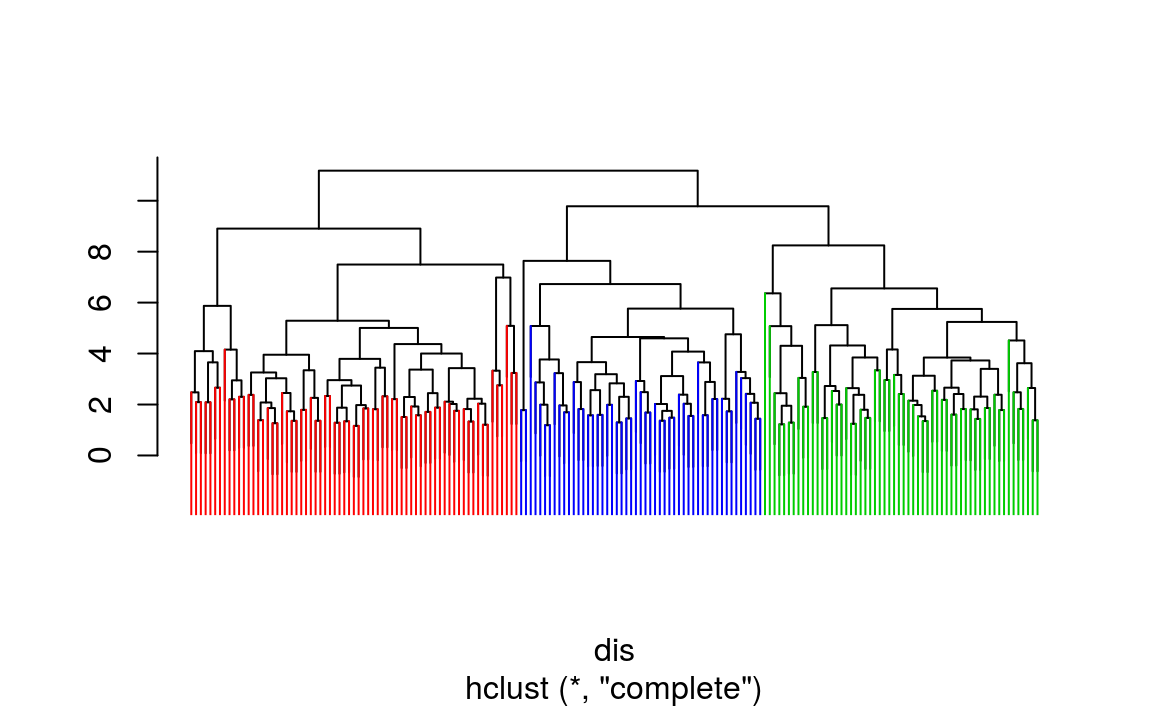
\includegraphics[width=0.5\linewidth]{02-regression_files/figure-latex/unnamed-chunk-20-1} \end{center}

피처가 3개로 구성된 모형이 가장 작은 Cp 값을 가집니다.

\begin{Shaded}
\begin{Highlighting}[]
\KeywordTok{plot}\NormalTok{(reg.sub, }\DataTypeTok{scale =} \StringTok{'Cp'}\NormalTok{)}
\end{Highlighting}
\end{Shaded}

\begin{center}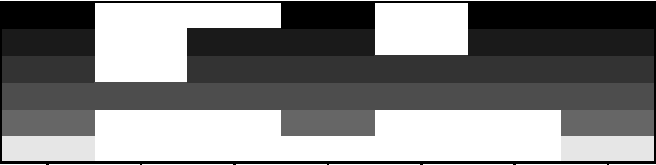
\includegraphics[width=0.5\linewidth]{02-regression_files/figure-latex/unnamed-chunk-21-1} \end{center}

가장 작은 Cp 값을 제공하는 피처를 나타내고 있으며 \textbf{APSLAKE, OPRC, OPSLAKE}가 이 모형에 포함된 피처들입니다.

위에서 선택된 피처만으로 다중 회귀분석을 실시하도록 하겠습니다.

\begin{Shaded}
\begin{Highlighting}[]
\NormalTok{reg.best =}\StringTok{ }\KeywordTok{lm}\NormalTok{(BSAAM }\OperatorTok{~}\StringTok{ }\NormalTok{APSLAKE }\OperatorTok{+}\StringTok{ }\NormalTok{OPRC }\OperatorTok{+}\StringTok{ }\NormalTok{OPSLAKE, }\DataTypeTok{data =}\NormalTok{ socal.water) }
\KeywordTok{summary}\NormalTok{(reg.best)}
\end{Highlighting}
\end{Shaded}

\begin{verbatim}
## 
## Call:
## lm(formula = BSAAM ~ APSLAKE + OPRC + OPSLAKE, data = socal.water)
## 
## Residuals:
##    Min     1Q Median     3Q    Max 
## -12964  -5140  -1252   4446  18649 
## 
## Coefficients:
##             Estimate Std. Error t value  Pr(>|t|)    
## (Intercept)    15425       3638    4.24   0.00013 ***
## APSLAKE         1712        500    3.42   0.00148 ** 
## OPRC            1798        568    3.17   0.00300 ** 
## OPSLAKE         2390        447    5.35 0.0000042 ***
## ---
## Signif. codes:  
## 0 '***' 0.001 '**' 0.01 '*' 0.05 '.' 0.1 ' ' 1
## 
## Residual standard error: 7280 on 39 degrees of freedom
## Multiple R-squared:  0.924,  Adjusted R-squared:  0.919 
## F-statistic:  159 on 3 and 39 DF,  p-value: <2e-16
\end{verbatim}

3개의 피처만으로 회귀분석한 \(R^2\)가 0.9185로써, 전체 피처로 회귀분석한 \(R^2\)인 0.9123 대비 증가합니다.

\begin{Shaded}
\begin{Highlighting}[]
\KeywordTok{par}\NormalTok{(}\DataTypeTok{mfrow =} \KeywordTok{c}\NormalTok{(}\DecValTok{2}\NormalTok{, }\DecValTok{2}\NormalTok{))}
\KeywordTok{plot}\NormalTok{(reg.best)}
\end{Highlighting}
\end{Shaded}

\begin{center}\includegraphics[width=0.5\linewidth]{02-regression_files/figure-latex/unnamed-chunk-23-1} \end{center}

\hypertarget{robustness-check}{%
\subsection{Robustness Check}\label{robustness-check}}

회귀분석의 가정이 맞는지 강건성 체크를 해보도록 하겠습니다.

\hypertarget{uxb2e4uxc911uxacf5uxc120uxc131}{%
\subsubsection{다중공선성}\label{uxb2e4uxc911uxacf5uxc120uxc131}}

다중공선성(multicollinearity) 여부를 조사하기 위해서는 분산 팽창 인자(VIF: Variance inflation factor) 통계량을 사용해야 합니다. VIF는 모든 피처가 들어 있는 전체 모형을 적합화할 때 계산된 특정한 피처 계수의 분산과 그 피처만 들어 있는 부분 모형으로 적합화했을 때의 계수 분산의 비율입니다.

\[VIF = 1 / (1 - R^2_i)\]

car 패키지의 \texttt{vif()} 함수를 통해 해당 값을 계산할 수 있습니다.

\begin{Shaded}
\begin{Highlighting}[]
\KeywordTok{vif}\NormalTok{(reg.best)}
\end{Highlighting}
\end{Shaded}

\begin{verbatim}
## APSLAKE    OPRC OPSLAKE 
##   1.011   6.453   6.445
\end{verbatim}

OPRC과 OPSLAKE의 vif가 매우 높게 나오며, 이는 OPRC와 OPSLAKE 간 상관관계가 지나치게 높기 때문입니다.

\begin{Shaded}
\begin{Highlighting}[]
\KeywordTok{plot}\NormalTok{(socal.water}\OperatorTok{$}\NormalTok{OPRC, socal.water}\OperatorTok{$}\NormalTok{OPSLAKE,}
     \DataTypeTok{xlab =} \StringTok{'OPRC'}\NormalTok{, }\DataTypeTok{ylab =} \StringTok{'OPSLAKE'}\NormalTok{)}
\end{Highlighting}
\end{Shaded}

\begin{center}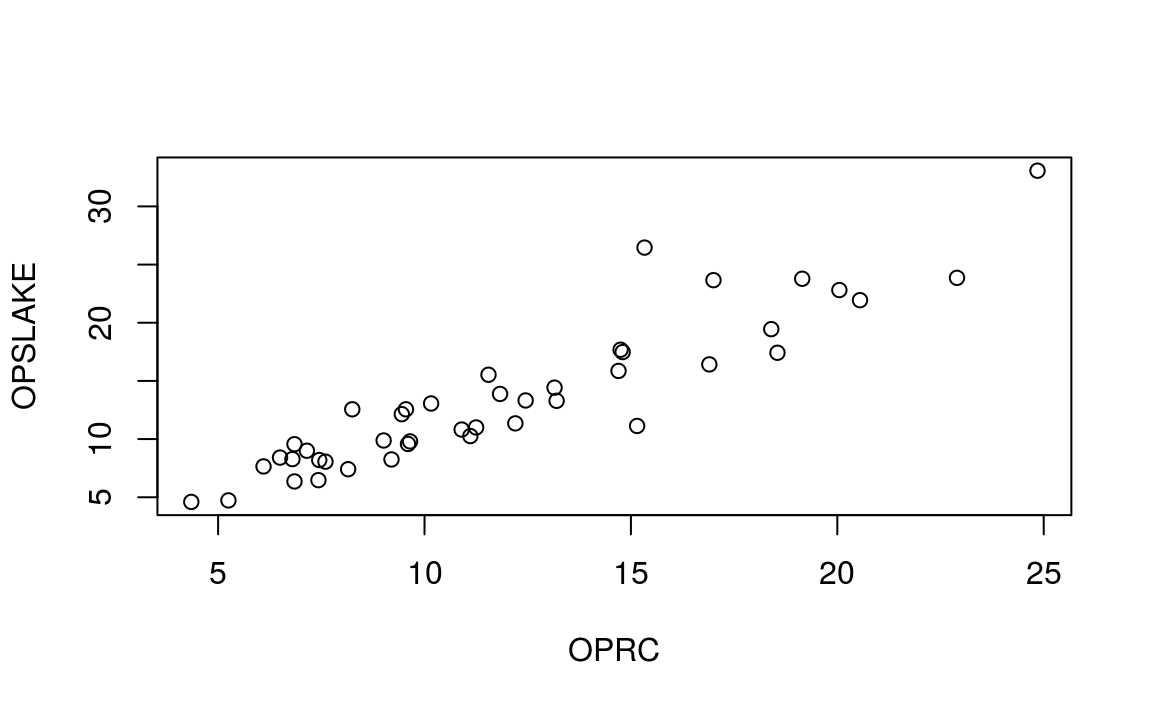
\includegraphics[width=0.5\linewidth]{02-regression_files/figure-latex/unnamed-chunk-25-1} \end{center}

따라서 둘 중 하나의 변수를 탈락시키는 것이 좋습니다.

\begin{Shaded}
\begin{Highlighting}[]
\NormalTok{best.summary}\OperatorTok{$}\NormalTok{adjr2}
\end{Highlighting}
\end{Shaded}

\begin{verbatim}
## [1] 0.8778 0.9002 0.9185 0.9169 0.9147 0.9123
\end{verbatim}

변수가 2개인 경우 \(R^2\)는 0.900이며, 3개인 경우 \(R^2\)는 0.918여서 증가가 경미합니다. 변수 2개로만 이뤄진 모형의 가정을 점검합니다.

\begin{Shaded}
\begin{Highlighting}[]
\NormalTok{fit}\FloatTok{.2}\NormalTok{ =}\StringTok{ }\KeywordTok{lm}\NormalTok{(BSAAM }\OperatorTok{~}\StringTok{ }\NormalTok{APSLAKE }\OperatorTok{+}\StringTok{ }\NormalTok{OPSLAKE, }\DataTypeTok{data =}\NormalTok{ socal.water)}
\KeywordTok{summary}\NormalTok{(fit}\FloatTok{.2}\NormalTok{)}
\end{Highlighting}
\end{Shaded}

\begin{verbatim}
## 
## Call:
## lm(formula = BSAAM ~ APSLAKE + OPSLAKE, data = socal.water)
## 
## Residuals:
##    Min     1Q Median     3Q    Max 
## -13336  -5893   -172   4220  19500 
## 
## Coefficients:
##             Estimate Std. Error t value Pr(>|t|)    
## (Intercept)    19145       3812    5.02 0.000011 ***
## APSLAKE         1769        554    3.19   0.0027 ** 
## OPSLAKE         3690        196   18.83  < 2e-16 ***
## ---
## Signif. codes:  
## 0 '***' 0.001 '**' 0.01 '*' 0.05 '.' 0.1 ' ' 1
## 
## Residual standard error: 8060 on 40 degrees of freedom
## Multiple R-squared:  0.905,  Adjusted R-squared:   0.9 
## F-statistic:  190 on 2 and 40 DF,  p-value: <2e-16
\end{verbatim}

\begin{Shaded}
\begin{Highlighting}[]
\KeywordTok{par}\NormalTok{(}\DataTypeTok{mfrow =} \KeywordTok{c}\NormalTok{(}\DecValTok{2}\NormalTok{, }\DecValTok{2}\NormalTok{))}
\KeywordTok{plot}\NormalTok{(fit}\FloatTok{.2}\NormalTok{)}

\KeywordTok{vif}\NormalTok{(fit}\FloatTok{.2}\NormalTok{)}
\end{Highlighting}
\end{Shaded}

\begin{verbatim}
## APSLAKE OPSLAKE 
##    1.01    1.01
\end{verbatim}

\begin{center}
\includegraphics[width=0.5\linewidth]{02-regression_files/figure-latex/unnamed-chunk-27-1} \end{center}

\hypertarget{uxb4f1uxbd84uxc0b0uxc131}{%
\subsubsection{등분산성}\label{uxb4f1uxbd84uxc0b0uxc131}}

등분산성에 여부는 브루시-페이건(Breusch-Pagan, BP) 테스트를 통해 확인이 가능하며, lmtest 패키지의 \texttt{bptest()} 함수를 이용합니다.

\begin{Shaded}
\begin{Highlighting}[]
\KeywordTok{library}\NormalTok{(lmtest)}
\KeywordTok{bptest}\NormalTok{(fit}\FloatTok{.2}\NormalTok{)}
\end{Highlighting}
\end{Shaded}

\begin{verbatim}
## 
##  studentized Breusch-Pagan test
## 
## data:  fit.2
## BP = 0.0046, df = 2, p-value = 1
\end{verbatim}

BP 테스트의 귀무가설과 대립가설은 다음과 같습니다

\begin{itemize}
\tightlist
\item
  귀무가설: ``오차항은 등분산성을 띤다''
\item
  대립가설: ``오차항은 이분산성을 띤다''
\end{itemize}

p 값이 0.9977로 매우크므로 귀무가설을 기각할 근거가 부족해, 오차항은 등분산을 띤다는 것을 알 수 있습니다.

\hypertarget{uxc2e4uxc81cuxc640-uxc608uxce21uxac04uxc758-uxcc28uxc774}{%
\subsection{실제와 예측간의 차이}\label{uxc2e4uxc81cuxc640-uxc608uxce21uxac04uxc758-uxcc28uxc774}}

\textbf{model\$fitted.values}에는 모델을 통해 나온 예측값이 있으므로, 실제 값과 차이를 살펴볼 수 있습니다.

\begin{Shaded}
\begin{Highlighting}[]
\KeywordTok{plot}\NormalTok{(fit}\FloatTok{.2}\OperatorTok{$}\NormalTok{fitted.values, socal.water}\OperatorTok{$}\NormalTok{BSAAM, }
     \DataTypeTok{xlab =} \StringTok{'predicted'}\NormalTok{, }\DataTypeTok{ylab =} \StringTok{'actual'}\NormalTok{, }\DataTypeTok{main =} \StringTok{'Predicted vs. Actual'}\NormalTok{)}
\end{Highlighting}
\end{Shaded}

\begin{center}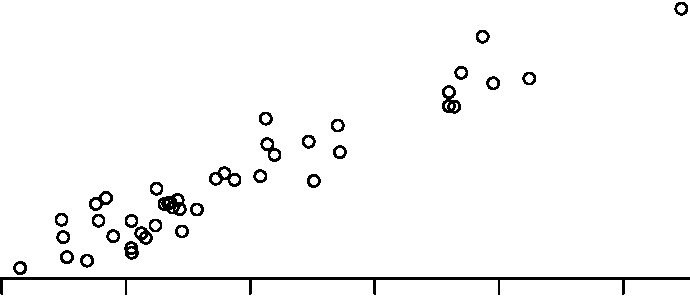
\includegraphics[width=0.5\linewidth]{02-regression_files/figure-latex/unnamed-chunk-29-1} \end{center}

ggplot을 이용 이용하면 더욱 깔끔하게 이를 나타낼 수 있다.

\begin{Shaded}
\begin{Highlighting}[]
\KeywordTok{library}\NormalTok{(ggplot2)}
\KeywordTok{library}\NormalTok{(magrittr)}

\NormalTok{socal.water[}\StringTok{'Actual'}\NormalTok{] =}\StringTok{ }\NormalTok{water}\OperatorTok{$}\NormalTok{BSAAM}
\NormalTok{socal.water}\OperatorTok{$}\NormalTok{Forecast =}\StringTok{ }\KeywordTok{predict}\NormalTok{(fit}\FloatTok{.2}\NormalTok{)}

\NormalTok{socal.water }\OperatorTok
\StringTok{  }\KeywordTok{ggplot}\NormalTok{(}\KeywordTok{aes}\NormalTok{(}\DataTypeTok{x =}\NormalTok{ Forecast, }\DataTypeTok{y =}\NormalTok{ Actual)) }\OperatorTok{+}\StringTok{ }
\StringTok{  }\KeywordTok{geom_point}\NormalTok{() }\OperatorTok{+}
\StringTok{  }\KeywordTok{geom_smooth}\NormalTok{(}\DataTypeTok{method =} \StringTok{'lm'}\NormalTok{, }\DataTypeTok{se =} \OtherTok{FALSE}\NormalTok{) }\OperatorTok{+}
\StringTok{  }\KeywordTok{labs}\NormalTok{(}\DataTypeTok{title =} \StringTok{'Forecast vs. Actuals'}\NormalTok{)}
\end{Highlighting}
\end{Shaded}

\begin{center}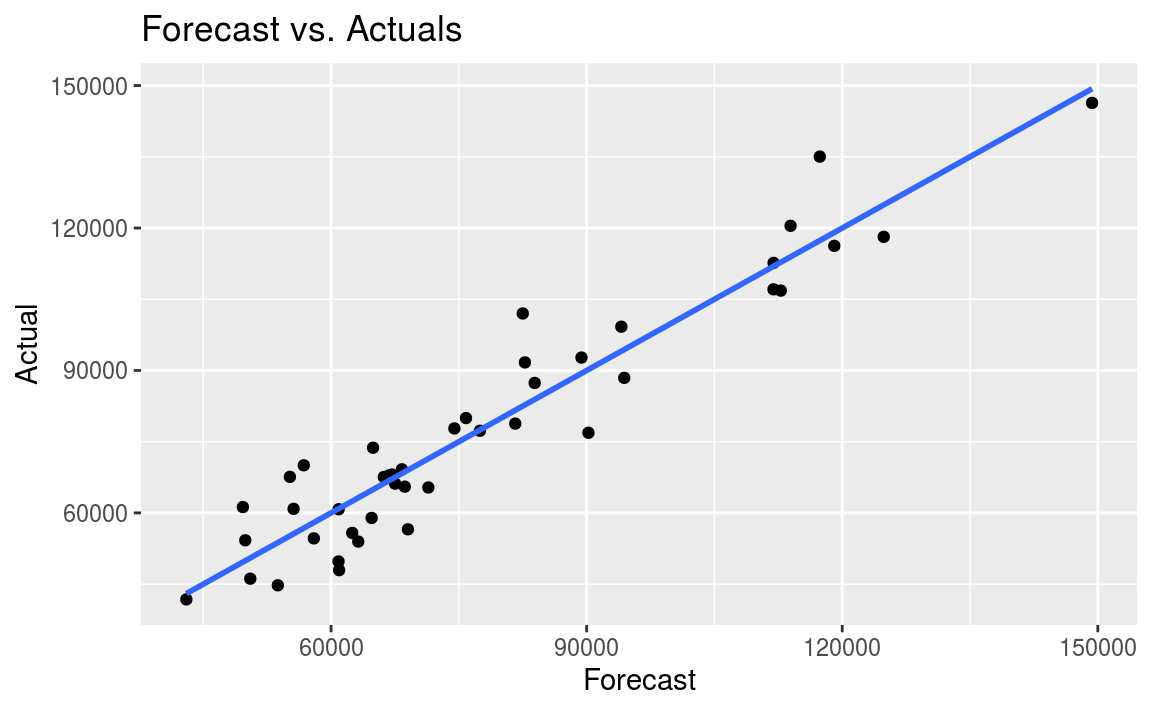
\includegraphics[width=0.5\linewidth]{02-regression_files/figure-latex/unnamed-chunk-30-1} \end{center}

\hypertarget{uxb2e4uxb978-uxace0uxb824uxc0acuxd56d}{%
\section{다른 고려사항}\label{uxb2e4uxb978-uxace0uxb824uxc0acuxd56d}}

\hypertarget{uxc9c8uxc801-uxd53cuxcc98}{%
\subsection{질적 피처}\label{uxc9c8uxc801-uxd53cuxcc98}}

질적 피처(qualitative feature)에서는 남성/여성 또는 나쁨/중간/좋음 등 2개나 그 이상의 단계를 정할 수 있습니다.

예를 들어 성별처럼 두 가지 단계를 갖는 피처가 있다면, 지표 혹은 더미 피처라는 변수를 만들어 임의로 단계 하나는 0, 다른 하나는 1로 줄 수 있습니다. 지표만을 이용해 모형을 만들어도 여전히 선형 모형은 기존 식과 같습니다.

\[Y = B_0 + B_1x + e\]

피처가 남성일 때 0, 여성일 때 1로 할당할 경우, 남성의 기대값은 \(y\) 절편인 \(B_0\)이고, 여성의 기대값은 \(B_0 + B_1x\) 입니다. R 내에서 factor 형태로 된 피처를 사용할 경우 자동으로 질적 피처로 계산이 됩니다.

예제로 ISLR 패키지의 Carseats 데이터 세트를 사용하도록 합니다.

\begin{Shaded}
\begin{Highlighting}[]
\KeywordTok{library}\NormalTok{(ISLR)}
\KeywordTok{data}\NormalTok{(Carseats)}
\KeywordTok{str}\NormalTok{(Carseats)}
\end{Highlighting}
\end{Shaded}

\begin{verbatim}
## 'data.frame':    400 obs. of  11 variables:
##  $ Sales      : num  9.5 11.22 10.06 7.4 4.15 ...
##  $ CompPrice  : num  138 111 113 117 141 124 115 136 132 132 ...
##  $ Income     : num  73 48 35 100 64 113 105 81 110 113 ...
##  $ Advertising: num  11 16 10 4 3 13 0 15 0 0 ...
##  $ Population : num  276 260 269 466 340 501 45 425 108 131 ...
##  $ Price      : num  120 83 80 97 128 72 108 120 124 124 ...
##  $ ShelveLoc  : Factor w/ 3 levels "Bad","Good","Medium": 1 2 3 3 1 1 3 2 3 3 ...
##  $ Age        : num  42 65 59 55 38 78 71 67 76 76 ...
##  $ Education  : num  17 10 12 14 13 16 15 10 10 17 ...
##  $ Urban      : Factor w/ 2 levels "No","Yes": 2 2 2 2 2 1 2 2 1 1 ...
##  $ US         : Factor w/ 2 levels "No","Yes": 2 2 2 2 1 2 1 2 1 2 ...
\end{verbatim}

해당 데이터 중 정량적 피처인 광고(Advertising)과 질적 피처인 진열대 위치(ShelveLoc)만을 이용해 카시트(Carseats)의 판매량을 예측합니다. 이 중 진열대 위치는 Bad, Good, Medium 총 3개 level로 구성되어 있습니다.

\begin{Shaded}
\begin{Highlighting}[]
\NormalTok{sales.fit =}\StringTok{ }\KeywordTok{lm}\NormalTok{(Sales }\OperatorTok{~}\StringTok{ }\NormalTok{Advertising }\OperatorTok{+}\StringTok{ }\NormalTok{ShelveLoc, }\DataTypeTok{data =}\NormalTok{ Carseats)}
\KeywordTok{summary}\NormalTok{(sales.fit)}
\end{Highlighting}
\end{Shaded}

\begin{verbatim}
## 
## Call:
## lm(formula = Sales ~ Advertising + ShelveLoc, data = Carseats)
## 
## Residuals:
##    Min     1Q Median     3Q    Max 
## -6.648 -1.620 -0.048  1.531  6.410 
## 
## Coefficients:
##                 Estimate Std. Error t value Pr(>|t|)
## (Intercept)       4.8966     0.2521   19.43  < 2e-16
## Advertising       0.1007     0.0169    5.95  5.9e-09
## ShelveLocGood     4.5769     0.3348   13.67  < 2e-16
## ShelveLocMedium   1.7514     0.2748    6.37  5.1e-10
##                    
## (Intercept)     ***
## Advertising     ***
## ShelveLocGood   ***
## ShelveLocMedium ***
## ---
## Signif. codes:  
## 0 '***' 0.001 '**' 0.01 '*' 0.05 '.' 0.1 ' ' 1
## 
## Residual standard error: 2.24 on 396 degrees of freedom
## Multiple R-squared:  0.373,  Adjusted R-squared:  0.369 
## F-statistic: 78.6 on 3 and 396 DF,  p-value: <2e-16
\end{verbatim}

진열대 위치가 좋은 경우(ShelveLocGood)는 위치가 나쁜 경우의 판매량인 Intercept 값인 4.89662 대비 4.57686이 더 높습니다.

\hypertarget{uxc0c1uxd638uxc791uxc6a9-uxd56d}{%
\subsection{상호작용 항}\label{uxc0c1uxd638uxc791uxc6a9-uxd56d}}

어떤 피처가 예측에 미치는 영향이 또 다른 피처에 종속적일 경우, 이 두 피처는 서로 상호작용한다고 말합니다.

\[Y = B_0 + B_1x + B_2 + B_1B_2x + e\]

MASS 패키지의 Boston 데이터 세트를 이용해 상호작용 회귀분석을 살펴보도록 하겠습니다.

\begin{Shaded}
\begin{Highlighting}[]
\KeywordTok{library}\NormalTok{(MASS)}
\KeywordTok{data}\NormalTok{(Boston)}
\KeywordTok{str}\NormalTok{(Boston)}
\end{Highlighting}
\end{Shaded}

\begin{verbatim}
## 'data.frame':    506 obs. of  14 variables:
##  $ crim   : num  0.00632 0.02731 0.02729 0.03237 0.06905 ...
##  $ zn     : num  18 0 0 0 0 0 12.5 12.5 12.5 12.5 ...
##  $ indus  : num  2.31 7.07 7.07 2.18 2.18 2.18 7.87 7.87 7.87 7.87 ...
##  $ chas   : int  0 0 0 0 0 0 0 0 0 0 ...
##  $ nox    : num  0.538 0.469 0.469 0.458 0.458 0.458 0.524 0.524 0.524 0.524 ...
##  $ rm     : num  6.58 6.42 7.18 7 7.15 ...
##  $ age    : num  65.2 78.9 61.1 45.8 54.2 58.7 66.6 96.1 100 85.9 ...
##  $ dis    : num  4.09 4.97 4.97 6.06 6.06 ...
##  $ rad    : int  1 2 2 3 3 3 5 5 5 5 ...
##  $ tax    : num  296 242 242 222 222 222 311 311 311 311 ...
##  $ ptratio: num  15.3 17.8 17.8 18.7 18.7 18.7 15.2 15.2 15.2 15.2 ...
##  $ black  : num  397 397 393 395 397 ...
##  $ lstat  : num  4.98 9.14 4.03 2.94 5.33 ...
##  $ medv   : num  24 21.6 34.7 33.4 36.2 28.7 22.9 27.1 16.5 18.9 ...
\end{verbatim}

이 중 사용할 피처의 설명은 다음과 같습니다.

\begin{itemize}
\tightlist
\item
  medv: 주택 가치의 중위값
\item
  lstat: 낮은 사회 경제적 지위를 갖는 가구의 백분율
\item
  age: 주택의 연령
\end{itemize}

\texttt{lm()} 함수에 \(feature1 * feature2\)를 쓰면, 각 피처뿐만 아니라 두 피처의 상호작용 항도 모형에 포함됩니다.

\begin{Shaded}
\begin{Highlighting}[]
\NormalTok{value.fit =}\StringTok{ }\KeywordTok{lm}\NormalTok{(medv }\OperatorTok{~}\StringTok{ }\NormalTok{lstat }\OperatorTok{*}\StringTok{ }\NormalTok{age, }\DataTypeTok{data =}\NormalTok{ Boston)}
\KeywordTok{summary}\NormalTok{(value.fit)}
\end{Highlighting}
\end{Shaded}

\begin{verbatim}
## 
## Call:
## lm(formula = medv ~ lstat * age, data = Boston)
## 
## Residuals:
##    Min     1Q Median     3Q    Max 
## -15.81  -4.04  -1.33   2.08  27.55 
## 
## Coefficients:
##              Estimate Std. Error t value Pr(>|t|)    
## (Intercept) 36.088536   1.469835   24.55  < 2e-16 ***
## lstat       -1.392117   0.167456   -8.31  8.8e-16 ***
## age         -0.000721   0.019879   -0.04    0.971    
## lstat:age    0.004156   0.001852    2.24    0.025 *  
## ---
## Signif. codes:  
## 0 '***' 0.001 '**' 0.01 '*' 0.05 '.' 0.1 ' ' 1
## 
## Residual standard error: 6.15 on 502 degrees of freedom
## Multiple R-squared:  0.556,  Adjusted R-squared:  0.553 
## F-statistic:  209 on 3 and 502 DF,  p-value: <2e-16
\end{verbatim}

lstat은 매우 예측력이 높은 피처이며, age는 예측력이 높지 않습니다. 그러나 이 두 피처는 유의한 상호작용을 보이며, medv를 설명하는 변수입니다.

\hypertarget{uxb85cuxc9c0uxc2a4uxd2f1-uxd68cuxadc0}{%
\chapter{로지스틱 회귀}\label{uxb85cuxc9c0uxc2a4uxd2f1-uxd68cuxadc0}}

\hypertarget{uxc624uxc988uxbe44}{%
\section{오즈비}\label{uxc624uxc988uxbe44}}

오즈는 성공할 확률이 실패할 확률의 몇 배인지를 나타내는 것으로써, \(Probability(Y) / 1 - (Probability(Y))\) 공식을 통해 계산됩니다. 예를 들어, 브라질이 월드컵 경기에서 이길 확률이 20\%라면, 오즈는 \(0.2 / (1-0.2) = 0.25\)가 되고, 1대 4의 승산입니다. 오즈를 확률로 역변환하려면 오즈를 \(1 + (오즈)\)로 나누며, 앞의 예에서는 \(0.25 / (1+0.25) = 0.2\), 즉 20\%가 됩니다.

만일 독일이 우승할 오즈가 0.18, 브라질이 우승할 오즈가 0.25인 경우 둘 간의 오즈를 오즈비를 이용해 비교할 수 있습니다. 브라질이 독일 대비 월드컵에서 우승할 확률은 0.25 / 0.18 = 1.39 입니다.

\hypertarget{uxb85cuxc9c0uxc2a4uxd2f1-uxd68cuxadc0-1}{%
\section{로지스틱 회귀}\label{uxb85cuxc9c0uxc2a4uxd2f1-uxd68cuxadc0-1}}

결과가 이항 혹은 다항 범주일 경우, 관찰값이 출력 변수의 특정 범주에 속할 확률을 예측해야 합니다. 이를 위해 기존 OLS 선형 회귀를 사용할 경우 매우 큰 측정 오차가 생길 수 있으며 편향된 결과를 낳습니다.

분류 문제는 0과 1 사이의 값을 갖는 확률로 가장 잘 모형화할 수 있습니다. 로지스틱 회귀와 선형 회귀의 관계는 로지스틱 회귀의 종속 변수를 로그 오즈, 즉 \(log(P(Y) / 1-P(Y))\)로 표현하고 이 값이 \(a + bX\)와 같음을 밝힘으로써 보일 수 있습니다. 이를 정리하면 다음과 같습니다.

\[log(\frac{P(Y)}{1-P(Y)}) = a + bX\]
\[\frac{P(Y)}{1-P(Y)} = e^{a + bX}\]
\[ P(Y) = \frac{e^{a + bX}}{1 + e^{a + bX}}  \]

위 \(P(Y)\) 를 그래프로 나타내면 다음과 같다.

\begin{center}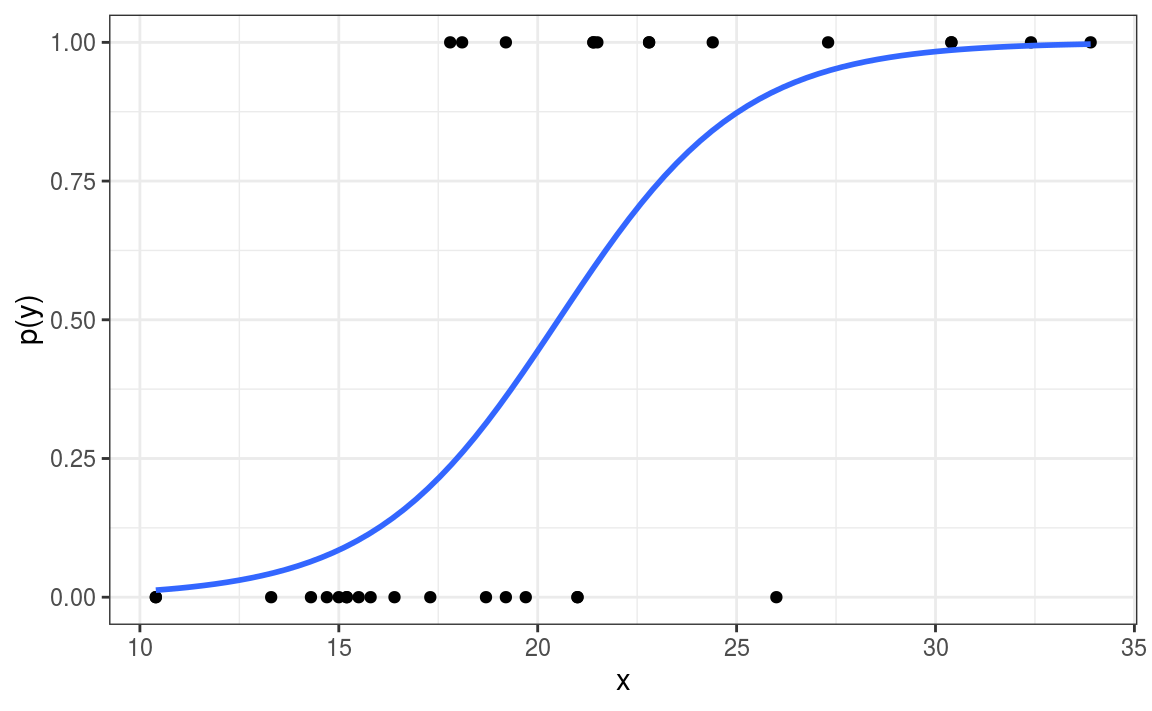
\includegraphics[width=0.5\linewidth]{03-logistic_files/figure-latex/unnamed-chunk-2-1} \end{center}

즉 \(x\)에 따른 \(y\)의 확률이 0과 1 사이에 놓이게 됩니다.

\hypertarget{uxc785uxd559-uxb370uxc774uxd130-uxbd84uxc11d}{%
\section{입학 데이터 분석}\label{uxc785uxd559-uxb370uxc774uxd130-uxbd84uxc11d}}

GRE, GPA, RANK가 입학(admission)에 어떤 영향을 주는지 로지스틱 회귀분석을 통해 분석하도록 하겠습니다.

\begin{Shaded}
\begin{Highlighting}[]
\NormalTok{admission =}\StringTok{ }\KeywordTok{read.csv}\NormalTok{(}\StringTok{"https://stats.idre.ucla.edu/stat/data/binary.csv"}\NormalTok{)}
\KeywordTok{head}\NormalTok{(admission)}
\end{Highlighting}
\end{Shaded}

\begin{verbatim}
##   admit gre  gpa rank
## 1     0 380 3.61    3
## 2     1 660 3.67    3
## 3     1 800 4.00    1
## 4     1 640 3.19    4
## 5     0 520 2.93    4
## 6     1 760 3.00    2
\end{verbatim}

\texttt{glm()} 함수를 이용하여 로지스틱 회귀분석을 실시합니다.

\begin{Shaded}
\begin{Highlighting}[]
\NormalTok{ad.logit =}\StringTok{ }\KeywordTok{glm}\NormalTok{(admit }\OperatorTok{~}\StringTok{ }\NormalTok{., }\DataTypeTok{family =}\NormalTok{ binomial, }\DataTypeTok{data =}\NormalTok{ admission)}
\KeywordTok{summary}\NormalTok{(ad.logit)}
\end{Highlighting}
\end{Shaded}

\begin{verbatim}
## 
## Call:
## glm(formula = admit ~ ., family = binomial, data = admission)
## 
## Deviance Residuals: 
##    Min      1Q  Median      3Q     Max  
## -1.580  -0.885  -0.638   1.157   2.173  
## 
## Coefficients:
##             Estimate Std. Error z value Pr(>|z|)    
## (Intercept) -3.44955    1.13285   -3.05   0.0023 ** 
## gre          0.00229    0.00109    2.10   0.0356 *  
## gpa          0.77701    0.32748    2.37   0.0177 *  
## rank        -0.56003    0.12714   -4.40 0.000011 ***
## ---
## Signif. codes:  
## 0 '***' 0.001 '**' 0.01 '*' 0.05 '.' 0.1 ' ' 1
## 
## (Dispersion parameter for binomial family taken to be 1)
## 
##     Null deviance: 499.98  on 399  degrees of freedom
## Residual deviance: 459.44  on 396  degrees of freedom
## AIC: 467.4
## 
## Number of Fisher Scoring iterations: 4
\end{verbatim}

모든 변수가 유의미한 결과를 보입니다. 로지스틱 회귀에서는 OLS와는 다르게 피처의 계수를 \(X\)가 한 단위 변화할 때 \(Y\)가 변화하는 양을 나타낸다고 해석할 수 없습니다. 로그 함수에서 \(\beta\)라는 계수는 오즈비 \(e^\beta\)로 변환해 해석해야 합니다.

\begin{Shaded}
\begin{Highlighting}[]
\KeywordTok{exp}\NormalTok{(}\KeywordTok{coef}\NormalTok{(ad.logit))}
\end{Highlighting}
\end{Shaded}

\begin{verbatim}
## (Intercept)         gre         gpa        rank 
##     0.03176     1.00230     2.17497     0.57119
\end{verbatim}

오즈비는 피처가 한 단위 변했을 때 나타나는 결과의 오지로 해석할 수 있습니다. 만일 이 값이 1보다 크면 피처가 증가할 때 결과의 오즈도 증가하며, 1보다 작으면 피처가 증가할 때 결과의 오즈는 감소합니다.

위의 예에서 gre와 gpa는 로그 오즈를 증가시키지만, rank는 로그 오즈를 감소시킵니다.

\begin{Shaded}
\begin{Highlighting}[]
\NormalTok{ad.probs =}\StringTok{ }\NormalTok{ad.logit}\OperatorTok{$}\NormalTok{fitted.values}
\NormalTok{ad.probs =}\StringTok{ }\KeywordTok{ifelse}\NormalTok{(ad.probs }\OperatorTok{>}\StringTok{ }\FloatTok{0.5}\NormalTok{, }\DecValTok{1}\NormalTok{, }\DecValTok{0}\NormalTok{)}
\end{Highlighting}
\end{Shaded}

회귀분석 결과의 fitted.values에는 확률이 저장되어 있으며, 해당 값이 0.5보다 크면 1, 그렇지 않으면 0로 변환해줍니다. 이를 실제 데이터와 비교해보도록 합니다.

\begin{Shaded}
\begin{Highlighting}[]
\KeywordTok{table}\NormalTok{(ad.probs, admission}\OperatorTok{$}\NormalTok{admit)}
\end{Highlighting}
\end{Shaded}

\begin{verbatim}
##         
## ad.probs   0   1
##        0 253  98
##        1  20  29
\end{verbatim}

\begin{Shaded}
\begin{Highlighting}[]
\KeywordTok{prop.table}\NormalTok{(}\KeywordTok{table}\NormalTok{(ad.probs, admission}\OperatorTok{$}\NormalTok{admit))}
\end{Highlighting}
\end{Shaded}

\begin{verbatim}
##         
## ad.probs      0      1
##        0 0.6325 0.2450
##        1 0.0500 0.0725
\end{verbatim}

맞게 판단할 확률이 대략 70\% 입니다.

\hypertarget{uxc704uxc2a4uxcf58uxc2e0-uxc720uxbc29uxc554-uxb370uxc774uxd130}{%
\section{위스콘신 유방암 데이터}\label{uxc704uxc2a4uxcf58uxc2e0-uxc720uxbc29uxc554-uxb370uxc774uxd130}}

위스콘신 유방암 데이터를 통해 종양이 양성 혹은 악성인지에 대해 예측해보도록 하겠습니다. 해당 데이터는 MASS 패키지의 \texttt{biopsy} 이름으로 저장되어 있습니다.

\hypertarget{uxb370uxc774uxd130-uxbd88uxb7ecuxc624uxae30-uxbc0f-uxd3b8uxc9d1}{%
\subsection{데이터 불러오기 및 편집}\label{uxb370uxc774uxd130-uxbd88uxb7ecuxc624uxae30-uxbc0f-uxd3b8uxc9d1}}

\begin{Shaded}
\begin{Highlighting}[]
\KeywordTok{library}\NormalTok{(MASS)}

\KeywordTok{data}\NormalTok{(biopsy)}
\KeywordTok{str}\NormalTok{(biopsy)}
\end{Highlighting}
\end{Shaded}

\begin{verbatim}
## 'data.frame':    699 obs. of  11 variables:
##  $ ID   : chr  "1000025" "1002945" "1015425" "1016277" ...
##  $ V1   : int  5 5 3 6 4 8 1 2 2 4 ...
##  $ V2   : int  1 4 1 8 1 10 1 1 1 2 ...
##  $ V3   : int  1 4 1 8 1 10 1 2 1 1 ...
##  $ V4   : int  1 5 1 1 3 8 1 1 1 1 ...
##  $ V5   : int  2 7 2 3 2 7 2 2 2 2 ...
##  $ V6   : int  1 10 2 4 1 10 10 1 1 1 ...
##  $ V7   : int  3 3 3 3 3 9 3 3 1 2 ...
##  $ V8   : int  1 2 1 7 1 7 1 1 1 1 ...
##  $ V9   : int  1 1 1 1 1 1 1 1 5 1 ...
##  $ class: Factor w/ 2 levels "benign","malignant": 1 1 1 1 1 2 1 1 1 1 ...
\end{verbatim}

각 피처는 다음과 같습니다.

\begin{itemize}
\tightlist
\item
  ID: 표본의 코드 번호
\item
  V1: 두께
\item
  V2: 세포 크기의 균일성
\item
  V3: 세포 모양의 균일성
\item
  V4: 한계 부착력
\item
  V5: 단일 상피세포 크기
\item
  V6: 나핵(16개의 관찰값 결측)
\item
  V7: 특징 없는 염색질
\item
  V8: 정상 핵소체
\item
  V9: 분열
\item
  class: 종양의 진단의 결과, 양성 또는 악성. 우리가 예측하려는 결과
\end{itemize}

피처명이 입력되어 있지 않으므로, 이를 입력해주도록 합니다.

\begin{Shaded}
\begin{Highlighting}[]
\NormalTok{biopsy}\OperatorTok{$}\NormalTok{ID =}\StringTok{ }\OtherTok{NULL}
\KeywordTok{names}\NormalTok{(biopsy) =}\StringTok{ }\KeywordTok{c}\NormalTok{(}\StringTok{'thick'}\NormalTok{, }\StringTok{'u.size'}\NormalTok{, }\StringTok{'u.shape'}\NormalTok{, }\StringTok{'adhsn'}\NormalTok{, }\StringTok{'s.size'}\NormalTok{,}
                  \StringTok{'nucl'}\NormalTok{, }\StringTok{'chrom'}\NormalTok{, }\StringTok{'n.nuc'}\NormalTok{, }\StringTok{'mit'}\NormalTok{, }\StringTok{'class'}\NormalTok{)}

\KeywordTok{head}\NormalTok{(biopsy)}
\end{Highlighting}
\end{Shaded}

\begin{verbatim}
##   thick u.size u.shape adhsn s.size nucl chrom n.nuc
## 1     5      1       1     1      2    1     3     1
## 2     5      4       4     5      7   10     3     2
## 3     3      1       1     1      2    2     3     1
## 4     6      8       8     1      3    4     3     7
## 5     4      1       1     3      2    1     3     1
## 6     8     10      10     8      7   10     9     7
##   mit     class
## 1   1    benign
## 2   1    benign
## 3   1    benign
## 4   1    benign
## 5   1    benign
## 6   1 malignant
\end{verbatim}

다음으로 결측 관측치를 삭제 및 데이터를 변형해줍니다.

\begin{Shaded}
\begin{Highlighting}[]
\KeywordTok{sum}\NormalTok{(}\KeywordTok{is.na}\NormalTok{(biopsy))}
\end{Highlighting}
\end{Shaded}

\begin{verbatim}
## [1] 16
\end{verbatim}

\begin{Shaded}
\begin{Highlighting}[]
\NormalTok{biopsy.v2 =}\StringTok{ }\KeywordTok{na.omit}\NormalTok{(biopsy)}
\NormalTok{y =}\StringTok{ }\KeywordTok{ifelse}\NormalTok{(biopsy.v2}\OperatorTok{$}\NormalTok{class }\OperatorTok{==}\StringTok{ 'malignant'}\NormalTok{, }\DecValTok{1}\NormalTok{, }\DecValTok{0}\NormalTok{)}
\KeywordTok{table}\NormalTok{(y)}
\end{Highlighting}
\end{Shaded}

\begin{verbatim}
## y
##   0   1 
## 444 239
\end{verbatim}

총 16개의 na 데이터가 존재하며, \texttt{na.omit()} 함수를 통해 해당 데이터를 모두 지워주도록 합니다. 또한 예측변수 y에는 class가 malignant(악성)일 경우 1, 그렇지 않을 경우 0을 입력합니다.

\texttt{gather()} 함수를 통해 테이블을 변경한 후, \texttt{ggplot()} 함수를 통해 각 class 별 피처들의 분포를 살펴보도록 합니다.

\begin{Shaded}
\begin{Highlighting}[]
\KeywordTok{library}\NormalTok{(ggplot2)}
\KeywordTok{library}\NormalTok{(dplyr)}
\KeywordTok{library}\NormalTok{(tidyr)}
\KeywordTok{library}\NormalTok{(magrittr)}

\NormalTok{biop.m =}\StringTok{ }\NormalTok{biopsy.v2 }\OperatorTok
\StringTok{  }\KeywordTok{gather}\NormalTok{(key, value, }\OperatorTok{-}\NormalTok{class)}

\NormalTok{biop.m }\OperatorTok
\StringTok{  }\KeywordTok{ggplot}\NormalTok{(}\KeywordTok{aes}\NormalTok{(}\DataTypeTok{x =}\NormalTok{ class, }\DataTypeTok{y =}\NormalTok{ value)) }\OperatorTok{+}\StringTok{ }
\StringTok{  }\KeywordTok{geom_boxplot}\NormalTok{() }\OperatorTok{+}
\StringTok{  }\KeywordTok{facet_wrap}\NormalTok{( }\OperatorTok{~}\StringTok{ }\NormalTok{key)}
\end{Highlighting}
\end{Shaded}

\begin{center}
\includegraphics[width=0.5\linewidth]{03-logistic_files/figure-latex/unnamed-chunk-11-1} \end{center}

다중공선성 확인을 위해 상관관계를 검사하도록 합니다.

\begin{Shaded}
\begin{Highlighting}[]
\KeywordTok{library}\NormalTok{(corrplot)}

\NormalTok{bc =}\StringTok{ }\NormalTok{biopsy.v2 }\OperatorTok
\StringTok{  }\NormalTok{dplyr}\OperatorTok{::}\KeywordTok{select}\NormalTok{(}\OperatorTok{-}\NormalTok{class) }\OperatorTok
\StringTok{  }\KeywordTok{cor}\NormalTok{()}

\KeywordTok{corrplot.mixed}\NormalTok{(bc)}
\end{Highlighting}
\end{Shaded}

\begin{center}\includegraphics[width=0.5\linewidth]{03-logistic_files/figure-latex/unnamed-chunk-12-1} \end{center}

u.size와 u.shape 간 상관관계가 0.91로 다중공선성 문제가 두드러져 보입니다.

\hypertarget{uxb370uxc774uxd130-uxb098uxb204uxae30}{%
\subsection{데이터 나누기}\label{uxb370uxc774uxd130-uxb098uxb204uxae30}}

기존에는 모든 데이터를 이용하여 모델을 훈련시켰습니다. 그러나 모델의 예측력을 평가하기 위해서는 모델링에 사용되지 않은 데이터와 평가하야 합니다. 이를 위해 트레이닝 및 테스트 세트로 나누도록 합니다. 일반적으로 트레이닝과 테스트 셋의 비율은 7:3 혹은 8:2로 합니다.

\begin{center}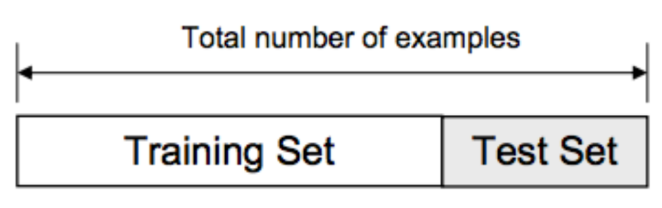
\includegraphics[width=0.5\linewidth]{images/data_split} \end{center}

\begin{Shaded}
\begin{Highlighting}[]
\KeywordTok{set.seed}\NormalTok{(}\DecValTok{123}\NormalTok{)}

\NormalTok{ind =}\StringTok{ }\KeywordTok{sample}\NormalTok{(}\DecValTok{2}\NormalTok{, }\KeywordTok{nrow}\NormalTok{(biopsy.v2), }\DataTypeTok{replace =} \OtherTok{TRUE}\NormalTok{,}
             \DataTypeTok{prob =} \KeywordTok{c}\NormalTok{(}\FloatTok{0.7}\NormalTok{, }\FloatTok{0.3}\NormalTok{))}

\NormalTok{train =}\StringTok{ }\NormalTok{biopsy.v2[ind}\OperatorTok{==}\DecValTok{1}\NormalTok{, ]}
\NormalTok{test =}\StringTok{ }\NormalTok{biopsy.v2[ind}\OperatorTok{==}\DecValTok{2}\NormalTok{, ]}
\end{Highlighting}
\end{Shaded}

\begin{Shaded}
\begin{Highlighting}[]
\KeywordTok{prop.table}\NormalTok{(}\KeywordTok{table}\NormalTok{(train}\OperatorTok{$}\NormalTok{class))}
\end{Highlighting}
\end{Shaded}

\begin{verbatim}
## 
##    benign malignant 
##    0.6371    0.3629
\end{verbatim}

\begin{Shaded}
\begin{Highlighting}[]
\KeywordTok{prop.table}\NormalTok{(}\KeywordTok{table}\NormalTok{(test}\OperatorTok{$}\NormalTok{class))}
\end{Highlighting}
\end{Shaded}

\begin{verbatim}
## 
##    benign malignant 
##    0.6794    0.3206
\end{verbatim}

\texttt{sample()} 을 통해 무작위 숫자를 7:3 비율로 생성한 후, train과 test 셋으로 나눠주도록 합니다. 그 후 각 데이터 셋의 종속변수의 비율을 확인해 7:3 비율과 비슷한지 확인합니다.

\hypertarget{uxbaa8uxd615uxd654}{%
\subsection{모형화}\label{uxbaa8uxd615uxd654}}

먼저 모든 입력 변수로 로지스틱 모형을 만든 후 점차 줄여 나가며 최량 부분 집합을 생성하도록 합니다.

\begin{Shaded}
\begin{Highlighting}[]
\NormalTok{full.fit =}\StringTok{ }\KeywordTok{glm}\NormalTok{(class }\OperatorTok{~}\StringTok{ }\NormalTok{., }\DataTypeTok{family =}\NormalTok{ binomial, }\DataTypeTok{data =}\NormalTok{ train)}
\KeywordTok{summary}\NormalTok{(full.fit)}
\end{Highlighting}
\end{Shaded}

\begin{verbatim}
## 
## Call:
## glm(formula = class ~ ., family = binomial, data = train)
## 
## Deviance Residuals: 
##    Min      1Q  Median      3Q     Max  
## -3.340  -0.139  -0.072   0.032   2.356  
## 
## Coefficients:
##             Estimate Std. Error z value Pr(>|z|)    
## (Intercept)   -9.429      1.227   -7.68  1.6e-14 ***
## thick          0.525      0.160    3.28  0.00104 ** 
## u.size        -0.105      0.245   -0.43  0.66917    
## u.shape        0.280      0.253    1.11  0.26804    
## adhsn          0.309      0.174    1.78  0.07572 .  
## s.size         0.287      0.207    1.38  0.16702    
## nucl           0.406      0.121    3.34  0.00083 ***
## chrom          0.274      0.217    1.26  0.20801    
## n.nuc          0.224      0.137    1.63  0.10213    
## mit            0.430      0.339    1.27  0.20540    
## ---
## Signif. codes:  
## 0 '***' 0.001 '**' 0.01 '*' 0.05 '.' 0.1 ' ' 1
## 
## (Dispersion parameter for binomial family taken to be 1)
## 
##     Null deviance: 620.989  on 473  degrees of freedom
## Residual deviance:  78.373  on 464  degrees of freedom
## AIC: 98.37
## 
## Number of Fisher Scoring iterations: 8
\end{verbatim}

\begin{Shaded}
\begin{Highlighting}[]
\KeywordTok{exp}\NormalTok{(}\KeywordTok{coef}\NormalTok{(full.fit)) }\OperatorTok\StringTok{ }\KeywordTok{round}\NormalTok{(., }\DecValTok{4}\NormalTok{)}
\end{Highlighting}
\end{Shaded}

\begin{verbatim}
## (Intercept)       thick      u.size     u.shape 
##      0.0001      1.6909      0.9007      1.3228 
##       adhsn      s.size        nucl       chrom 
##      1.3615      1.3319      1.5003      1.3148 
##       n.nuc         mit 
##      1.2516      1.5367
\end{verbatim}

위 예제에서 u.size를 제외한 모든 피처가 로그 오즈를 증가시킵니다. 다음으로 다중공선성을 확인합니다.

\begin{Shaded}
\begin{Highlighting}[]
\KeywordTok{library}\NormalTok{(car)}
\KeywordTok{vif}\NormalTok{(full.fit)}
\end{Highlighting}
\end{Shaded}

\begin{verbatim}
##   thick  u.size u.shape   adhsn  s.size    nucl   chrom 
##   1.235   3.249   2.830   1.302   1.636   1.373   1.523 
##   n.nuc     mit 
##   1.343   1.060
\end{verbatim}

위의 값들 중 어느 것도 통계값이 5보다 크지 않으므로 공선성을 크게 문제가 되지 안습니다.

\begin{Shaded}
\begin{Highlighting}[]
\NormalTok{train.probs =}\StringTok{ }\NormalTok{full.fit}\OperatorTok{$}\NormalTok{fitted.values}
\KeywordTok{head}\NormalTok{(train.probs)}
\end{Highlighting}
\end{Shaded}

\begin{verbatim}
##       1       3       6       7       9      10 
## 0.02053 0.01088 0.99993 0.08987 0.01379 0.00842
\end{verbatim}

확률을 선택한 후, 해당 값이 0.5보다 클 경우 1, 아닐 경우 0으로 구분합니다. 그 후 train 데이터의 class와 비교하여 예측 정확도를 비교해보도록 한다.

\begin{Shaded}
\begin{Highlighting}[]
\NormalTok{train.bi =}\StringTok{ }\KeywordTok{ifelse}\NormalTok{(train.probs }\OperatorTok{>}\StringTok{ }\FloatTok{0.5}\NormalTok{, }\DecValTok{1}\NormalTok{, }\DecValTok{0}\NormalTok{) }\OperatorTok\StringTok{ }\KeywordTok{as.factor}\NormalTok{()}
\NormalTok{train.class =}\StringTok{ }\KeywordTok{ifelse}\NormalTok{(train}\OperatorTok{$}\NormalTok{class }\OperatorTok{==}\StringTok{ 'malignant'}\NormalTok{, }\DecValTok{1}\NormalTok{, }\DecValTok{0}\NormalTok{) }\OperatorTok\StringTok{ }\KeywordTok{as.factor}\NormalTok{()}

\NormalTok{true.ratio =}\StringTok{ }\KeywordTok{prop.table}\NormalTok{(}\KeywordTok{table}\NormalTok{(train.bi, train.class))}
\KeywordTok{print}\NormalTok{(true.ratio[}\DecValTok{1}\NormalTok{,}\DecValTok{1}\NormalTok{] }\OperatorTok{+}\StringTok{ }\NormalTok{true.ratio[}\DecValTok{2}\NormalTok{,}\DecValTok{2}\NormalTok{])}
\end{Highlighting}
\end{Shaded}

\begin{verbatim}
## [1] 0.9684
\end{verbatim}

예측 정확도가 0.6203, 0.0169, 0.0148, 0.3481로 매우 높게 나타납니다.

\hypertarget{uxd63cuxb3c8-uxd589uxb82cconfusion-matrix-uxc774uxd574uxd558uxae30}{%
\subsubsection{혼돈 행렬(Confusion Matrix) 이해하기}\label{uxd63cuxb3c8-uxd589uxb82cconfusion-matrix-uxc774uxd574uxd558uxae30}}

혼돈 행렬은 예측 값이 실제 값과 일치하는지에 따라 여측을 범주화한 표입니다. 한 차원은 예측 값을 나타내고, 다른 차원은 실제값을 나타냅니다.

일반적으로 관심 있는 클래스를 positive 클래스, 다른 클래스들을 false 클래스라고 하며, 두 클래스의 관계는 네 종류의 범주 중 예측이 속하는 범주를 도표화한 2 X 2 혼동 행렬로 표현할 수 있습니다.

\begin{center}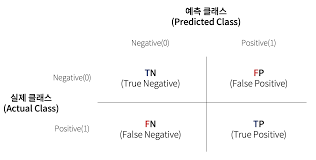
\includegraphics[width=0.5\linewidth]{images/confusion_matrix} \end{center}

각 항목의 설명은 다음과 같습니다.

\begin{itemize}
\tightlist
\item
  True Positive: 관심 클래스로 정확하게 분류
\item
  True Negative: 관심 클래스가 아닌 클래스로 정확하게 분류
\item
  False Positive: 관심 클래스로 부정확학 분류
\item
  False Negative: 관심 클래스가 아닌 클래스로 부정확하게 분류
\end{itemize}

혼돈 행렬을 이용한 성능 측정에는 다음과 같은 값들이 있습니다.

\begin{itemize}
\item
  \textbf{정확도(Accuracy)}: \(\frac{TP + TN}{TP + TN + FP + FN}\), True Positive과 True Negative의 횟수를 전체 예측 횟수로 나눈 값
\item
  오류율(Error rate): \(\frac{FP + FN}{TP + TN + FP + FN} = 1 - 정확도\), 부정확한 분류된 예시
\item
  재현율(Recall): \(\frac{TP}{TP + FN}\), True Postiive 개수를 전체 긍정 개수로 나누어 계산. 민감도(Sensitivity)로도 불림
\item
  특이도(Specificity, 참 부정률): \(\frac{TN}{TN + FP}\), True Negative의 개수를 전체 부정으로 나누어 계산
\item
  정밀도(Precision, 긍정 예측 값): \(\frac{TP}{TP + FP}\), 모델이 Positive로 예측할 때 예측이 얼마나 정확한지 여부
\item
  F 점수(F-score): \(\frac{2 \times 정밀도 \times 재현율}{재현율 + 정밀도} = \frac{2 \times TP}{2 \times TP + FP+ FN}\), 조화 평균을 이용하여 정밀도와 재현율을 결합
\end{itemize}

혼돈 행렬은 caret 패키지의 \texttt{confusionMatrix(predict,\ truth)} 함수를 이용해 계산할 수 있습니다.

\begin{Shaded}
\begin{Highlighting}[]
\NormalTok{caret}\OperatorTok{::}\KeywordTok{confusionMatrix}\NormalTok{(train.bi, train.class)}
\end{Highlighting}
\end{Shaded}

\begin{verbatim}
## Confusion Matrix and Statistics
## 
##           Reference
## Prediction   0   1
##          0 294   7
##          1   8 165
##                                         
##                Accuracy : 0.968         
##                  95% CI : (0.948, 0.982)
##     No Information Rate : 0.637         
##     P-Value [Acc > NIR] : <2e-16        
##                                         
##                   Kappa : 0.932         
##                                         
##  Mcnemar's Test P-Value : 1             
##                                         
##             Sensitivity : 0.974         
##             Specificity : 0.959         
##          Pos Pred Value : 0.977         
##          Neg Pred Value : 0.954         
##              Prevalence : 0.637         
##          Detection Rate : 0.620         
##    Detection Prevalence : 0.635         
##       Balanced Accuracy : 0.966         
##                                         
##        'Positive' Class : 0             
## 
\end{verbatim}

정확도를 의미하는 \emph{Accuracy}가 0.9684로 직접 계산한 값과 동일합니다.

\hypertarget{uxd14cuxc2a4uxd2b8-uxc14buxc5d0-uxc801uxc6a9}{%
\subsection{테스트 셋에 적용}\label{uxd14cuxc2a4uxd2b8-uxc14buxc5d0-uxc801uxc6a9}}

위 모형은 트레이닝 셋을 대상으로 만들어졌습니다. 따라서 모형에 포함되지 않은 데이터인 테스트 셋의 데이터를 대상으로 모델의 정확도를 구해보도록 합니다.

\begin{Shaded}
\begin{Highlighting}[]
\NormalTok{test.probs =}\StringTok{ }\KeywordTok{predict}\NormalTok{(full.fit, }\DataTypeTok{newdata =}\NormalTok{ test, }\DataTypeTok{type =} \StringTok{'response'}\NormalTok{)}

\NormalTok{test.bi =}\StringTok{ }\KeywordTok{ifelse}\NormalTok{(test.probs }\OperatorTok{>}\StringTok{ }\FloatTok{0.5}\NormalTok{, }\DecValTok{1}\NormalTok{, }\DecValTok{0}\NormalTok{) }\OperatorTok\StringTok{ }\KeywordTok{as.factor}\NormalTok{()}
\NormalTok{test.class =}\StringTok{ }\KeywordTok{ifelse}\NormalTok{(test}\OperatorTok{$}\NormalTok{class }\OperatorTok{==}\StringTok{ 'malignant'}\NormalTok{, }\DecValTok{1}\NormalTok{, }\DecValTok{0}\NormalTok{) }\OperatorTok\StringTok{ }\KeywordTok{as.factor}\NormalTok{()}

\NormalTok{caret}\OperatorTok{::}\KeywordTok{confusionMatrix}\NormalTok{(test.bi, test.class)}
\end{Highlighting}
\end{Shaded}

\begin{verbatim}
## Confusion Matrix and Statistics
## 
##           Reference
## Prediction   0   1
##          0 139   2
##          1   3  65
##                                         
##                Accuracy : 0.976         
##                  95% CI : (0.945, 0.992)
##     No Information Rate : 0.679         
##     P-Value [Acc > NIR] : <2e-16        
##                                         
##                   Kappa : 0.945         
##                                         
##  Mcnemar's Test P-Value : 1             
##                                         
##             Sensitivity : 0.979         
##             Specificity : 0.970         
##          Pos Pred Value : 0.986         
##          Neg Pred Value : 0.956         
##              Prevalence : 0.679         
##          Detection Rate : 0.665         
##    Detection Prevalence : 0.675         
##       Balanced Accuracy : 0.975         
##                                         
##        'Positive' Class : 0             
## 
\end{verbatim}

\texttt{predict()} 함수의 newdata 인자에 test를 입력하여 확률을 계산한 후, 혼돈 행렬을 구하도록 합니다. 정확도가 0.9761로써 역시나 뛰어난 성과를 보입니다.

\hypertarget{uxad50uxcc28uxac80uxc99duxc744-uxd3ecuxd568uxd55c-uxb85cuxc9c0uxc2a4uxd2f1-uxd68cuxadc0}{%
\section{교차검증을 포함한 로지스틱 회귀}\label{uxad50uxcc28uxac80uxc99duxc744-uxd3ecuxd568uxd55c-uxb85cuxc9c0uxc2a4uxd2f1-uxd68cuxadc0}}

K-폴드 교차검증은 데이터 세트를 같은 크기를 갖는 조각으로 K등분한 후, K-세트 중에 1개의 세트를 번갈아 제외하며 학습합니다.

\begin{center}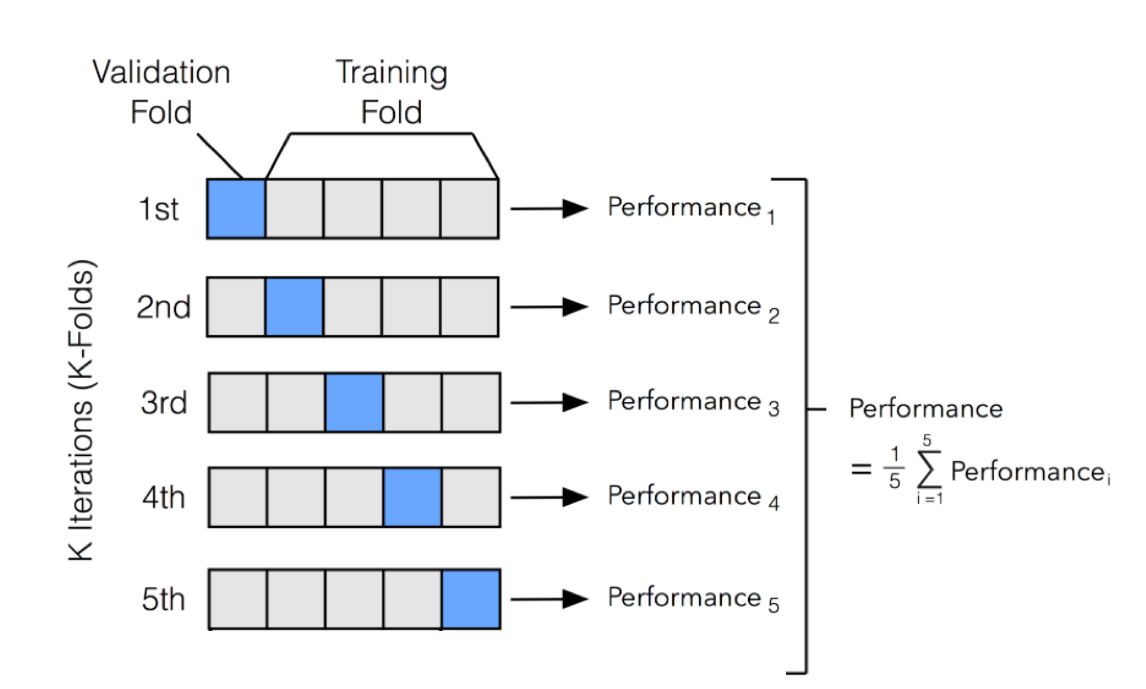
\includegraphics[width=0.5\linewidth]{images/kfolds} \end{center}

bestglm 패키지를 이용하여 교차 검증을 이용한 로지스틱 회귀분석을 실행할 수 있습니다. 해당 패키지를 이용하기 위해서 결과값을 0과 1로 코드화할 필요가 있으며, 만일 변수형이 팩터 형태로 남아 있으면 작동이 되지 않습니다. 또한 결과값인 \(y\)가 맨 마지막 컬럼에 위치해야 하며, 불필요한 컬럼은 삭제되어야 합니다.

이를 고려하여 새로운 데이터 테이블을 만들고, 교차 검증을 실시합니다.

\begin{Shaded}
\begin{Highlighting}[]
\KeywordTok{library}\NormalTok{(bestglm)}
\NormalTok{df =}\StringTok{ }\NormalTok{train }\OperatorTok
\StringTok{  }\KeywordTok{mutate}\NormalTok{(}\DataTypeTok{class =} \KeywordTok{ifelse}\NormalTok{(class }\OperatorTok{==}\StringTok{ 'malignant'}\NormalTok{, }\DecValTok{1}\NormalTok{, }\DecValTok{0}\NormalTok{))}

\KeywordTok{bestglm}\NormalTok{(df, }\DataTypeTok{IC =} \StringTok{'CV'}\NormalTok{,}
        \DataTypeTok{CVArgs =} \KeywordTok{list}\NormalTok{(}\DataTypeTok{Method =} \StringTok{'HTF'}\NormalTok{, }\DataTypeTok{K =} \DecValTok{10}\NormalTok{,}
                      \DataTypeTok{REP =} \DecValTok{1}\NormalTok{), }\DataTypeTok{family =}\NormalTok{ binomial)}
\end{Highlighting}
\end{Shaded}

\begin{verbatim}
## CV(K = 10, REP = 1)
## BICq equivalent for q in (0.0000716797006619085, 0.273173435514231)
## Best Model:
##             Estimate Std. Error z value  Pr(>|z|)
## (Intercept)  -7.8147    0.90996  -8.588 8.855e-18
## thick         0.6188    0.14713   4.206 2.598e-05
## u.size        0.6582    0.15295   4.303 1.683e-05
## nucl          0.5726    0.09923   5.771 7.899e-09
\end{verbatim}

K = 10 개를 대상으로 교차 검증을 수행한 결과 최적의 변수가 선택되었습니다. 해당 변수만을 이용하여 다시 로지스틱 회귀분석을 실시합니다.

\begin{Shaded}
\begin{Highlighting}[]
\NormalTok{reduce.fit =}\StringTok{ }\KeywordTok{glm}\NormalTok{(class }\OperatorTok{~}\StringTok{ }\NormalTok{thick }\OperatorTok{+}\StringTok{ }\NormalTok{u.size }\OperatorTok{+}\StringTok{ }\NormalTok{nucl, }\DataTypeTok{family =}\NormalTok{ binomial,}
                 \DataTypeTok{data =}\NormalTok{ train)}
\KeywordTok{summary}\NormalTok{(reduce.fit)}
\end{Highlighting}
\end{Shaded}

\begin{verbatim}
## 
## Call:
## glm(formula = class ~ thick + u.size + nucl, family = binomial, 
##     data = train)
## 
## Deviance Residuals: 
##    Min      1Q  Median      3Q     Max  
## -3.579  -0.181  -0.072   0.042   2.373  
## 
## Coefficients:
##             Estimate Std. Error z value     Pr(>|z|)
## (Intercept)  -7.8147     0.9100   -8.59      < 2e-16
## thick         0.6188     0.1471    4.21 0.0000259816
## u.size        0.6582     0.1530    4.30 0.0000168303
## nucl          0.5726     0.0992    5.77 0.0000000079
##                
## (Intercept) ***
## thick       ***
## u.size      ***
## nucl        ***
## ---
## Signif. codes:  
## 0 '***' 0.001 '**' 0.01 '*' 0.05 '.' 0.1 ' ' 1
## 
## (Dispersion parameter for binomial family taken to be 1)
## 
##     Null deviance: 620.989  on 473  degrees of freedom
## Residual deviance:  97.665  on 470  degrees of freedom
## AIC: 105.7
## 
## Number of Fisher Scoring iterations: 7
\end{verbatim}

위 모델을 테스트 셋에 적용한 후, 혼돈 행렬을 이용해 측값과 실제 값을 비교해보도록 합니다.

\begin{Shaded}
\begin{Highlighting}[]
\KeywordTok{library}\NormalTok{(caret)}

\NormalTok{test.cv.probs =}\StringTok{ }\KeywordTok{predict}\NormalTok{(reduce.fit, }\DataTypeTok{newdata =}\NormalTok{ test, }\DataTypeTok{type =} \StringTok{'response'}\NormalTok{)}
\NormalTok{test.cv.probs =}\StringTok{ }\KeywordTok{ifelse}\NormalTok{(test.cv.probs }\OperatorTok{>}\StringTok{ }\FloatTok{0.5}\NormalTok{, }\DecValTok{1}\NormalTok{, }\DecValTok{0}\NormalTok{) }\OperatorTok\StringTok{ }\KeywordTok{as.factor}\NormalTok{()}
\NormalTok{test.class =}\StringTok{ }\KeywordTok{ifelse}\NormalTok{(test}\OperatorTok{$}\NormalTok{class }\OperatorTok{==}\StringTok{ 'malignant'}\NormalTok{, }\DecValTok{1}\NormalTok{, }\DecValTok{0}\NormalTok{) }\OperatorTok\StringTok{ }\KeywordTok{as.factor}\NormalTok{()}

\NormalTok{caret}\OperatorTok{::}\KeywordTok{confusionMatrix}\NormalTok{(test.cv.probs, test.class)}
\end{Highlighting}
\end{Shaded}

\begin{verbatim}
## Confusion Matrix and Statistics
## 
##           Reference
## Prediction   0   1
##          0 139   5
##          1   3  62
##                                         
##                Accuracy : 0.962         
##                  95% CI : (0.926, 0.983)
##     No Information Rate : 0.679         
##     P-Value [Acc > NIR] : <2e-16        
##                                         
##                   Kappa : 0.911         
##                                         
##  Mcnemar's Test P-Value : 0.724         
##                                         
##             Sensitivity : 0.979         
##             Specificity : 0.925         
##          Pos Pred Value : 0.965         
##          Neg Pred Value : 0.954         
##              Prevalence : 0.679         
##          Detection Rate : 0.665         
##    Detection Prevalence : 0.689         
##       Balanced Accuracy : 0.952         
##                                         
##        'Positive' Class : 0             
## 
\end{verbatim}

모든 피처를 포함하는 모형에 비하면 정확도가 다소 떨어졌습니다.

\hypertarget{bic-uxae30uxc900-uxcd5cuxc801uxc758-uxd53cuxcc98-uxc120uxd0dd}{%
\section{BIC 기준 최적의 피처 선택}\label{bic-uxae30uxc900-uxcd5cuxc801uxc758-uxd53cuxcc98-uxc120uxd0dd}}

\texttt{bestglm()} 함수의 IC 인자를 변경하여 타 기준 최적 피처를 선택할 수 있으며, BIC 기준 최적의 피처를 선택하도로 하겠습니다.

\begin{Shaded}
\begin{Highlighting}[]
\KeywordTok{bestglm}\NormalTok{(df, }\DataTypeTok{IC =} \StringTok{'BIC'}\NormalTok{, }\DataTypeTok{family =}\NormalTok{ binomial)}
\end{Highlighting}
\end{Shaded}

\begin{verbatim}
## BIC
## BICq equivalent for q in (0.273173435514231, 0.577036596263764)
## Best Model:
##             Estimate Std. Error z value  Pr(>|z|)
## (Intercept)  -8.6170    1.03155  -8.353 6.633e-17
## thick         0.7114    0.14752   4.822 1.419e-06
## adhsn         0.4538    0.15034   3.018 2.541e-03
## nucl          0.5580    0.09848   5.666 1.462e-08
## n.nuc         0.4291    0.11846   3.622 2.920e-04
\end{verbatim}

이번에는 thick, adhsn, nucl, n.nuc 피처가 선택되었다. 이를 토대로 추정 및 정확도를 계산해봅니다.

\begin{Shaded}
\begin{Highlighting}[]
\NormalTok{bic.fit =}\StringTok{ }\KeywordTok{glm}\NormalTok{(class }\OperatorTok{~}\StringTok{ }\NormalTok{thick }\OperatorTok{+}\StringTok{ }\NormalTok{adhsn }\OperatorTok{+}\StringTok{ }\NormalTok{nucl }\OperatorTok{+}\StringTok{ }\NormalTok{n.nuc, }\DataTypeTok{family =}\NormalTok{ binomial,}
                 \DataTypeTok{data =}\NormalTok{ train)}

\NormalTok{test.bic.probs =}\StringTok{ }\KeywordTok{predict}\NormalTok{(bic.fit, }\DataTypeTok{newdata =}\NormalTok{ test, }\DataTypeTok{type =} \StringTok{'response'}\NormalTok{)}
\NormalTok{test.bic.probs =}\StringTok{ }\KeywordTok{ifelse}\NormalTok{(test.bic.probs }\OperatorTok{>}\StringTok{ }\FloatTok{0.5}\NormalTok{, }\DecValTok{1}\NormalTok{, }\DecValTok{0}\NormalTok{) }\OperatorTok\StringTok{ }\KeywordTok{as.factor}\NormalTok{()}

\NormalTok{caret}\OperatorTok{::}\KeywordTok{confusionMatrix}\NormalTok{(test.bic.probs, test.class)}
\end{Highlighting}
\end{Shaded}

\begin{verbatim}
## Confusion Matrix and Statistics
## 
##           Reference
## Prediction   0   1
##          0 138   1
##          1   4  66
##                                         
##                Accuracy : 0.976         
##                  95% CI : (0.945, 0.992)
##     No Information Rate : 0.679         
##     P-Value [Acc > NIR] : <2e-16        
##                                         
##                   Kappa : 0.946         
##                                         
##  Mcnemar's Test P-Value : 0.371         
##                                         
##             Sensitivity : 0.972         
##             Specificity : 0.985         
##          Pos Pred Value : 0.993         
##          Neg Pred Value : 0.943         
##              Prevalence : 0.679         
##          Detection Rate : 0.660         
##    Detection Prevalence : 0.665         
##       Balanced Accuracy : 0.978         
##                                         
##        'Positive' Class : 0             
## 
\end{verbatim}

정확도가 0.9761으로 소폭 개선되었습니다.

\hypertarget{roc}{%
\section{ROC}\label{roc}}

분류 모형을 선택할 때는 ROC(Receiver Operating Characteristic) 차트를 주로 이용합니다.

ROC 곡선은 거짓 긍정을 피하면서 참 긍정을 팀자하는 것 사이의 트레이드오프를 관찰하는데 사용되며, \(y\)축은 참 긍정율(TPR: True Positive Rate), \(x\)축은 거짓 긍정율(FPR: False Positive Rate)을 나타냅니다.

\[TPR = 긍정이라고\ 제대로\ 분류된 갯수 /\ 전체\ 긍정\ 갯수\]
\[FPR = 긍정이라고\ 잘못\ 분류된\ 부정\ 갯수 /\ 전체\ 부정\ 갯수\]
ROC 곡선을 구성하는 점들은 거짓 긍정의 임계치가 변화할 때 참 긍정률을 나타냅니다. 곡선을 생성하기 위해 분류기의 예측을 긍정 클래스의 추정 확률로 내림차순 정렬합니다. 원점에서 시작해 참 긍정률과 거짓 긍정률에 미치는 영향은 수직 또는 수평으로 추적하는 곡선을 만듭니다.

\begin{center}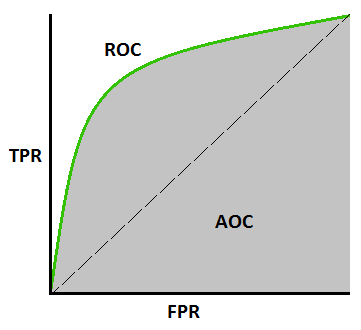
\includegraphics[width=0.5\linewidth]{images/roc} \end{center}

다이어그램의 왼쪽 하단 모서리에서 오른쪽 상단의 모서리까지 대각선은 예측 값이 없는 분류기를 나타냅니다 이 분류기는 참 긍정과 거짓 긍정이 정확히 같은 비율로 탐지되는데, 분류기가 이 둘을 구별하지 못한다는 것을 의미하며, 다른 분류기를 판단하기 위한 기준선입니다. 이 선에 가까운 ROC 곡선은 그다지 유용하지 않은 모델을 나타냅니다.

분류기가 완벽하다면 True Positive는 100\%, False Positive는 0\%인 y축과 같을 것입니다. 실제 분류기는 위 그림처럼 `완벽한' 분류기와 `쓸모없는' 분류기 사이의 영역에 위치할 것입니다.

ROC 곡선이 완벽한 분류기에 가까울수록 분류기는 Positive 값을 더욱 잘 식별하며, 이는 AUC (Area Under Curve)로 측정할 수 있습니다. AUC는 ROC 다이어그램을 2차원 정사각형으로 취급하며, ROC 곡선의 아래 전체 영역을 측정합니다. AUC는 0.5에서 1 사이 값을 나타냅니다.

다음은 모형의 ROC 및 AUC를 계산하는 방법입니다.

\begin{Shaded}
\begin{Highlighting}[]
\NormalTok{full.fit =}\StringTok{ }\KeywordTok{glm}\NormalTok{(class }\OperatorTok{~}\NormalTok{.,  }\DataTypeTok{family =}\NormalTok{ binomial, }\DataTypeTok{data =}\NormalTok{ train)}

\NormalTok{test.full.props =}\StringTok{ }\KeywordTok{predict}\NormalTok{(full.fit, }\DataTypeTok{newdata =}\NormalTok{ test, }\DataTypeTok{type =} \StringTok{'response'}\NormalTok{)}
\KeywordTok{head}\NormalTok{(test.full.props)}
\end{Highlighting}
\end{Shaded}

\begin{verbatim}
##        2        4        5        8       11       16 
## 0.960970 0.676287 0.022461 0.005702 0.001921 0.743727
\end{verbatim}

먼저 모든 피처로 로지스틱 회귀 분석을 실시한 후, \texttt{predict()} 함수를 이용해 테스트 셋에 모델을 적용합니다.

\begin{Shaded}
\begin{Highlighting}[]
\KeywordTok{library}\NormalTok{(InformationValue)}
\KeywordTok{plotROC}\NormalTok{(test.class, test.full.props)}
\end{Highlighting}
\end{Shaded}

\begin{center}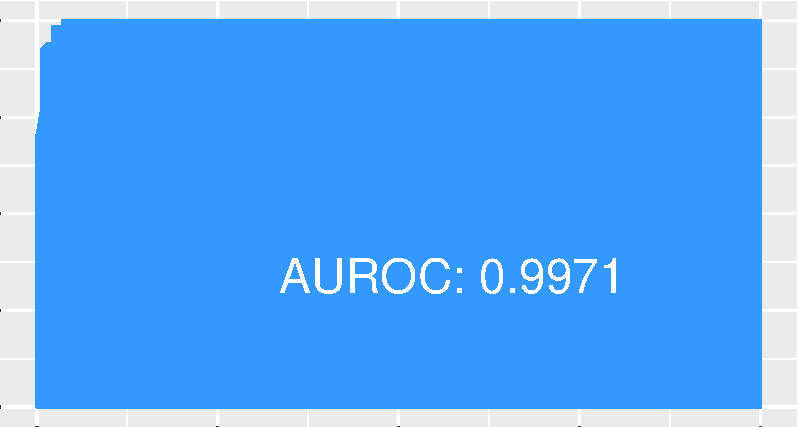
\includegraphics[width=0.5\linewidth]{03-logistic_files/figure-latex/unnamed-chunk-31-1} \end{center}

InformationValue 패키지의 \texttt{plotROC()} 함수를 이용해 ROC 그림 및 AUC 값을 계산할 수 있습니다.

\hypertarget{ridge-lasso}{%
\chapter{RIDGE \& LASSO}\label{ridge-lasso}}

\hypertarget{uxaddcuxc81cuxd654}{%
\section{규제화}\label{uxaddcuxc81cuxd654}}

선형 모형의 목적은 \(Y = B_o + B_1x_1 + \dots + B_nx_n + e\) 수식에서 RSS를 최소화 하는 것입니다. 규제화란 RSS를 최소화하는 과정에 벌점(\(\lambda\), Shrinkage penalty)을 적용합니다. 간단하게 말하면, 우리가 사용하는 모형에서는 앞으로 \(RSS + \lambda\)를 최소화합니다. 이 중 \(\lambda\)는 조정이 가능한 값이며, 해당 값이 0이면 OLS 모형과 같습니다.

\hypertarget{uxaddcuxc81cuxd654uxc758-uxc885uxb958}{%
\subsection{규제화의 종류}\label{uxaddcuxc81cuxd654uxc758-uxc885uxb958}}

규제화에는 일반적으로 두가지 방법이 사용됩니다.

\begin{itemize}
\item
  Ridge Regression: Ridge에서 사용하는 정규화 계수항은 가중값의 제곱 합으로, L2-norm 이라고도 부릅니다. 이 모델은 \(RSS + \lambda(\sum b_k^2)\)을 최소화하는 값입니다. 람다 값이 커질수록 계수는 0에 가까워지지만 0이 되지는 않습니다. 이는 예측의 정확성을 높이는 효과가 있지만, 어떠한 피처에 관한 가중값도 0으로 만들지 않기 때문에 모형을 해석하고 소통하는데 문제가 될 수도 있습니다.
\item
  LASSO: LASSO는 정규화한 계수항에 L1-norm을 사용합니다. L1-norm은 피처 가중값의 절대값의 합으로, \(RSS + \lambda(\sum |b_k|)\)를 최소화합니다. 이러한 벌점은 어떤 피처의 가중값을 0으로 만들 수도 있으며, 모형의 해석 능력을 크게 향상시킬 수 있습니다.
\end{itemize}

\hypertarget{uxc804uxb9bduxc120uxc554-uxb370uxc774uxd130-uxbd84uxc11d}{%
\section{전립선암 데이터 분석}\label{uxc804uxb9bduxc120uxc554-uxb370uxc774uxd130-uxbd84uxc11d}}

암-전립선암 데이터를 통해 규제화 기법을 사용한 차이를 살펴보도록 하겠습니다.

\hypertarget{uxb370uxc774uxd130-uxbd88uxb7ecuxc624uxae30-uxbc0f-uxd3b8uxc9d1-1}{%
\subsection{데이터 불러오기 및 편집}\label{uxb370uxc774uxd130-uxbd88uxb7ecuxc624uxae30-uxbc0f-uxd3b8uxc9d1-1}}

\begin{Shaded}
\begin{Highlighting}[]
\KeywordTok{library}\NormalTok{(ElemStatLearn) }\CommentTok{# 데이터}
\KeywordTok{library}\NormalTok{(car) }\CommentTok{# VIF 계싼}
\KeywordTok{library}\NormalTok{(corrplot)}
\KeywordTok{library}\NormalTok{(leaps) }\CommentTok{# 최량 부분 집합 회귀}
\KeywordTok{library}\NormalTok{(glmnet) }\CommentTok{# Ridge, Lasso}
\KeywordTok{library}\NormalTok{(caret)}

\KeywordTok{data}\NormalTok{(}\StringTok{"prostate"}\NormalTok{)}
\KeywordTok{str}\NormalTok{(prostate)}
\end{Highlighting}
\end{Shaded}

\begin{verbatim}
## 'data.frame':    97 obs. of  10 variables:
##  $ lcavol : num  -0.58 -0.994 -0.511 -1.204 0.751 ...
##  $ lweight: num  2.77 3.32 2.69 3.28 3.43 ...
##  $ age    : int  50 58 74 58 62 50 64 58 47 63 ...
##  $ lbph   : num  -1.39 -1.39 -1.39 -1.39 -1.39 ...
##  $ svi    : int  0 0 0 0 0 0 0 0 0 0 ...
##  $ lcp    : num  -1.39 -1.39 -1.39 -1.39 -1.39 ...
##  $ gleason: int  6 6 7 6 6 6 6 6 6 6 ...
##  $ pgg45  : int  0 0 20 0 0 0 0 0 0 0 ...
##  $ lpsa   : num  -0.431 -0.163 -0.163 -0.163 0.372 ...
##  $ train  : logi  TRUE TRUE TRUE TRUE TRUE TRUE ...
\end{verbatim}

각 피처는 다음과 같습니다.

\begin{itemize}
\tightlist
\item
  lcavol: 암 부피의 로그 값
\item
  lweight: 전립선 무게의 로그 값
\item
  age: 환자의 나이
\item
  lbph: 전립선 비대 크기의 로그 값
\item
  svi: 암 세포가 전립선 바깥에 있는 정낭에 침범했는지를 나타내는 변수, 1 = yes, 0 = no
\item
  lcp: 암 세포가 전립선 표면에서 얼마나 확장했고, 내부로 얼마나 침투했는지를 나타내는 로그 값
\item
  gleason: 암 세포가 얼마나 비정상적으로 보이는지 생체 검사를 통해 병리학자가 2에서 10 사이의 점수를 매긴 값. 이 점수가 높을수록 더 공격적인 암
\item
  pgg45: 글래슨 패턴 4 또는 5 (높은 단계의 암)
\item
  lpsa: PSA의 로그 값
\item
  train: 트레이닝, 테스트셋 데이터 여부
\end{itemize}

먼저 gleason의 분포를 확인해보도록 하겠습니다.

\begin{Shaded}
\begin{Highlighting}[]
\KeywordTok{table}\NormalTok{(prostate}\OperatorTok{$}\NormalTok{gleason)}
\end{Highlighting}
\end{Shaded}

\begin{verbatim}
## 
##  6  7  8  9 
## 35 56  1  5
\end{verbatim}

글리슨 점수가 6, 7점에 대부분 모여 있으며, 8점인 것은 1개, 9점인 것은 5개 밖에 없습니다. 해당 데이터 처리를 위해 다음과 같은 선택이 있습니다.

\begin{itemize}
\tightlist
\item
  해당 피처를 삭제
\item
  점수 8과 9만 삭제
\item
  해당 피처를 바꿔 새로운 변수를 만듬
\end{itemize}

이를 위해 글리슨 점수와 lpsa의 관계를 그림으로 살펴보도록 합니다.

\begin{Shaded}
\begin{Highlighting}[]
\KeywordTok{library}\NormalTok{(magrittr)}
\KeywordTok{library}\NormalTok{(ggplot2)}

\NormalTok{prostate }\OperatorTok
\StringTok{  }\KeywordTok{ggplot}\NormalTok{(}\KeywordTok{aes}\NormalTok{(}\DataTypeTok{x =}\NormalTok{ gleason, }\DataTypeTok{y =}\NormalTok{ lpsa, }\DataTypeTok{group =}\NormalTok{ gleason)) }\OperatorTok{+}
\StringTok{  }\KeywordTok{geom_boxplot}\NormalTok{() }
\end{Highlighting}
\end{Shaded}

\begin{center}\includegraphics[width=0.5\linewidth]{04-penalized_regression_files/figure-latex/unnamed-chunk-4-1} \end{center}

7\textasciitilde{}9점의 lpsa가 상당히 크므로, 피처를 남겨두는 것이 좋습니다. 따라서 글리슨 점수가 6점 일 때는 0, 7점 이상인 경우에는 1로 바꾸도록 합니다.

\begin{Shaded}
\begin{Highlighting}[]
\NormalTok{prostate}\OperatorTok{$}\NormalTok{gleason =}\StringTok{ }\KeywordTok{ifelse}\NormalTok{(prostate}\OperatorTok{$}\NormalTok{gleason }\OperatorTok{==}\StringTok{ }\DecValTok{6}\NormalTok{, }\DecValTok{0}\NormalTok{, }\DecValTok{1}\NormalTok{)}
\KeywordTok{table}\NormalTok{(prostate}\OperatorTok{$}\NormalTok{gleason)}
\end{Highlighting}
\end{Shaded}

\begin{verbatim}
## 
##  0  1 
## 35 62
\end{verbatim}

이번에는 각 피처간의 상관관계를 살펴보도록 합니다.

\begin{Shaded}
\begin{Highlighting}[]
\KeywordTok{cor}\NormalTok{(prostate) }\OperatorTok
\StringTok{  }\NormalTok{corrplot.mixed}
\end{Highlighting}
\end{Shaded}

\begin{center}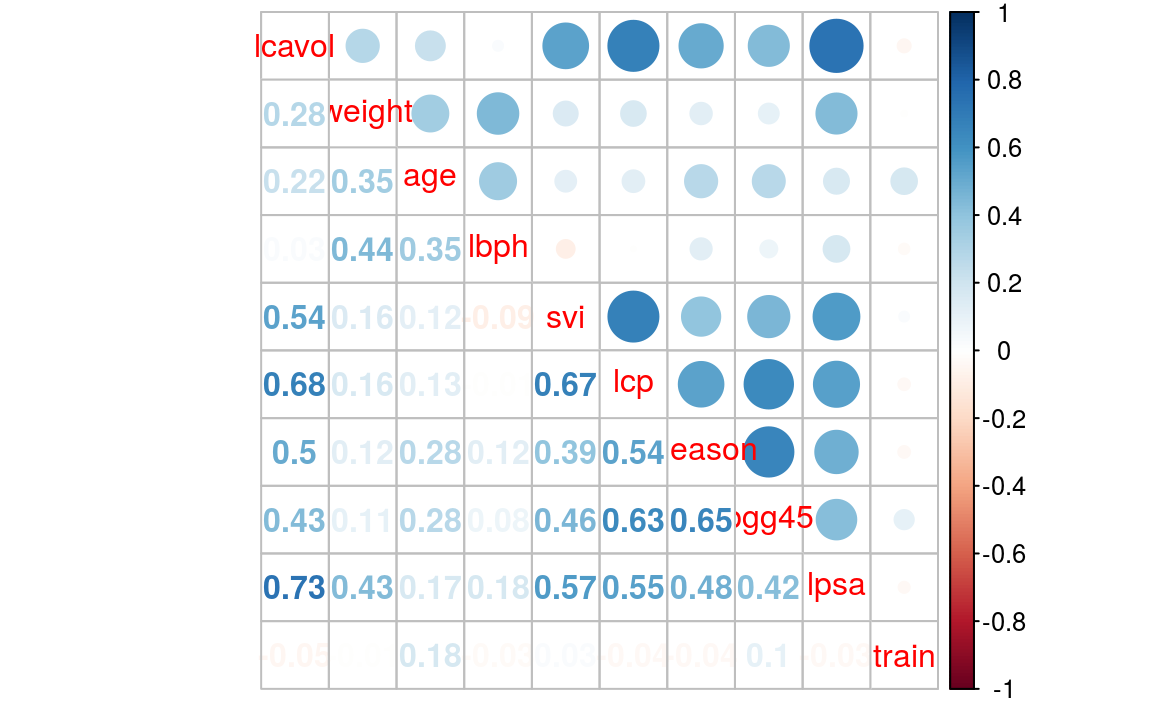
\includegraphics[width=0.5\linewidth]{04-penalized_regression_files/figure-latex/unnamed-chunk-6-1} \end{center}

lpsa와 lcavol, lcavol과 lcp, svi와 lcp 사이에는 상관관계가 높아 다중 공선성 문제가 발생할 수 있습니다.

\hypertarget{uxb370uxc774uxd130-uxb098uxb204uxae30-1}{%
\subsection{데이터 나누기}\label{uxb370uxc774uxd130-uxb098uxb204uxae30-1}}

다음으로 트레이닝 셋과 테스트 셋을 분리하도록 합니다.

\begin{Shaded}
\begin{Highlighting}[]
\NormalTok{train =}\StringTok{ }\KeywordTok{subset}\NormalTok{(prostate, train }\OperatorTok{==}\StringTok{ }\OtherTok{TRUE}\NormalTok{)[, }\DecValTok{1}\OperatorTok{:}\DecValTok{9}\NormalTok{]}
\NormalTok{test =}\StringTok{ }\KeywordTok{subset}\NormalTok{(prostate, train }\OperatorTok{==}\StringTok{ }\OtherTok{FALSE}\NormalTok{)[, }\DecValTok{1}\OperatorTok{:}\DecValTok{9}\NormalTok{]}
\end{Highlighting}
\end{Shaded}

train 열이 TRUE이면 트레이닝 셋, FALSE면 테스트 셋으로 나누어주도록 하며, 마지막 열인 train은 모형에 필요치 않으므로 이를 제외하고 선택해줍니다.

\hypertarget{uxbaa8uxd615uxd654-1}{%
\subsection{모형화}\label{uxbaa8uxd615uxd654-1}}

먼저 최량 부분 집합 회귀를 실시한 후 규제화 기법을 활용하도록 합니다.

\hypertarget{uxcd5cuxb7c9-uxbd80uxbd84-uxc9d1uxd569}{%
\subsubsection{최량 부분 집합}\label{uxcd5cuxb7c9-uxbd80uxbd84-uxc9d1uxd569}}

\texttt{regsubsets()} 함수를 이용해 최량 부분 집합 객체를 만듭니다.

\begin{Shaded}
\begin{Highlighting}[]
\NormalTok{subfit =}\StringTok{ }\KeywordTok{regsubsets}\NormalTok{(lpsa }\OperatorTok{~}\StringTok{ }\NormalTok{., }\DataTypeTok{data =}\NormalTok{ train)}

\NormalTok{b.sum =}\StringTok{ }\KeywordTok{summary}\NormalTok{(subfit)}
\KeywordTok{which.min}\NormalTok{(b.sum}\OperatorTok{$}\NormalTok{bic)}
\end{Highlighting}
\end{Shaded}

\begin{verbatim}
## [1] 3
\end{verbatim}

\begin{Shaded}
\begin{Highlighting}[]
\KeywordTok{plot}\NormalTok{(b.sum}\OperatorTok{$}\NormalTok{bic, }\DataTypeTok{type =} \StringTok{'l'}\NormalTok{, }\DataTypeTok{xlab =} \StringTok{'# of features'}\NormalTok{, }\DataTypeTok{ylab =} \StringTok{'BIC'}\NormalTok{)}
\end{Highlighting}
\end{Shaded}

\begin{center}\includegraphics[width=0.5\linewidth]{04-penalized_regression_files/figure-latex/unnamed-chunk-8-1} \end{center}

세 가지 피처를 사용한 모형이 가장 낮은 BIC를 보입니다. 도표를 통해 좀 더 자세하게 비교하도록 합니다.

\begin{Shaded}
\begin{Highlighting}[]
\KeywordTok{plot}\NormalTok{(subfit, }\DataTypeTok{scale =} \StringTok{'bic'}\NormalTok{)}
\end{Highlighting}
\end{Shaded}

\begin{center}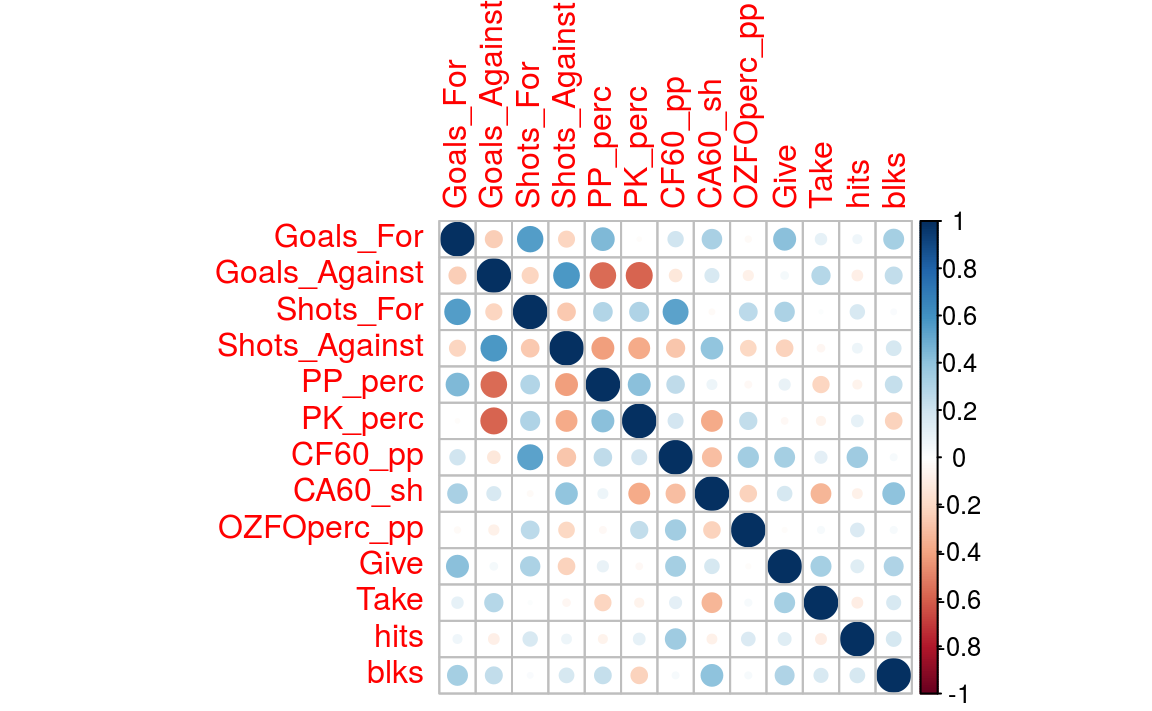
\includegraphics[width=0.5\linewidth]{04-penalized_regression_files/figure-latex/unnamed-chunk-9-1} \end{center}

lcavol, lweight, gleason 3개의 결합에서 가장 낮은 BIC를 보입니다. 이제 해당 모형을 통해 OLS 회귀분석을 실시합니다.

\begin{Shaded}
\begin{Highlighting}[]
\NormalTok{ols =}\StringTok{ }\KeywordTok{lm}\NormalTok{(lpsa }\OperatorTok{~}\StringTok{ }\NormalTok{lcavol }\OperatorTok{+}\StringTok{ }\NormalTok{lweight }\OperatorTok{+}\StringTok{ }\NormalTok{gleason, }\DataTypeTok{data =}\NormalTok{ train)}
\KeywordTok{plot}\NormalTok{(ols}\OperatorTok{$}\NormalTok{fitted.values, train}\OperatorTok{$}\NormalTok{lpsa, }\DataTypeTok{xlab =} \StringTok{'Predicted'}\NormalTok{, }\DataTypeTok{ylab =} \StringTok{'Actual'}\NormalTok{)}
\end{Highlighting}
\end{Shaded}

\begin{center}\includegraphics[width=0.5\linewidth]{04-penalized_regression_files/figure-latex/unnamed-chunk-10-1} \end{center}

둘 간에는 선형 관계가 보입니다. 이번에는 \texttt{predict()} 함수를 이용해 해당 모형을 테스트 셋에 적용해보도록 합니다.

\begin{Shaded}
\begin{Highlighting}[]
\NormalTok{pred.subfit =}\StringTok{ }\KeywordTok{predict}\NormalTok{(ols, }\DataTypeTok{newdata =}\NormalTok{ test)}
\KeywordTok{plot}\NormalTok{(pred.subfit, test}\OperatorTok{$}\NormalTok{lpsa, }\DataTypeTok{xlab =} \StringTok{'Predicted'}\NormalTok{, }\DataTypeTok{ylab =} \StringTok{'Actual'}\NormalTok{)}
\end{Highlighting}
\end{Shaded}

\begin{center}
\includegraphics[width=0.5\linewidth]{04-penalized_regression_files/figure-latex/unnamed-chunk-11-1} \end{center}

마지막으로 MSE를 계산하도록 합니다.

\begin{Shaded}
\begin{Highlighting}[]
\NormalTok{resid.subfit =}\StringTok{ }\NormalTok{test}\OperatorTok{$}\NormalTok{lpsa }\OperatorTok{-}\StringTok{ }\NormalTok{pred.subfit}
\NormalTok{mse.subfit =}\StringTok{ }\KeywordTok{mean}\NormalTok{(resid.subfit }\OperatorTok{^}\StringTok{ }\DecValTok{2}\NormalTok{)}
\KeywordTok{print}\NormalTok{(mse.subfit)}
\end{Highlighting}
\end{Shaded}

\begin{verbatim}
## [1] 0.5084
\end{verbatim}

위의 0.51 값을 기준으로 삼은 후, 규제화 기법과 비교하도록 하겠습니다.

\hypertarget{ridge-regression}{%
\subsubsection{Ridge Regression}\label{ridge-regression}}

\texttt{glmnet()} 함수를 이용해 Ridge 회귀분석을 수행할 수 있으며, 해당 함수는 입력 피처가 데이터 프레임이 아닌 행렬의 형태여야 합니다. 다음과 같은 형태로 함수를 입력합니다.

\[glmnet(x = 입력 데이터 행렬, y = 반응값, family = 분포 방법, alpha = 0)\]

이 중 alpha가 0이면 Ridge Regression, 1이면 LASSO 방법으로 분석을 합니다. 먼저 Ridge Regression을 수행합니다.

\begin{Shaded}
\begin{Highlighting}[]
\NormalTok{x =}\StringTok{ }\KeywordTok{as.matrix}\NormalTok{(train[, }\DecValTok{1}\OperatorTok{:}\DecValTok{8}\NormalTok{])}
\NormalTok{y =}\StringTok{ }\NormalTok{train[, }\DecValTok{9}\NormalTok{]}

\NormalTok{ridge =}\StringTok{ }\KeywordTok{glmnet}\NormalTok{(x, y, }\DataTypeTok{family =} \StringTok{'gaussian'}\NormalTok{, }\DataTypeTok{alpha =} \DecValTok{0}\NormalTok{)}
\end{Highlighting}
\end{Shaded}

\begin{Shaded}
\begin{Highlighting}[]
\KeywordTok{print}\NormalTok{(ridge)}
\end{Highlighting}
\end{Shaded}

\begin{center}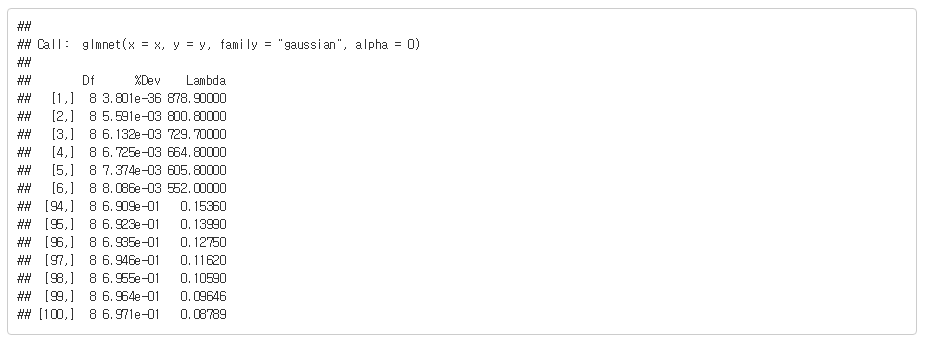
\includegraphics[width=1\linewidth]{images/ridge} \end{center}

마지막 100번째 결과를 살펴보면 사용하는 피처의 수가 여전히 8개입니다. 편차의 백분율은 0.6971이고, 람다 값은 0.08789 입니다.

\begin{Shaded}
\begin{Highlighting}[]
\KeywordTok{plot}\NormalTok{(ridge, }\DataTypeTok{label =} \OtherTok{TRUE}\NormalTok{)}
\end{Highlighting}
\end{Shaded}

\begin{center}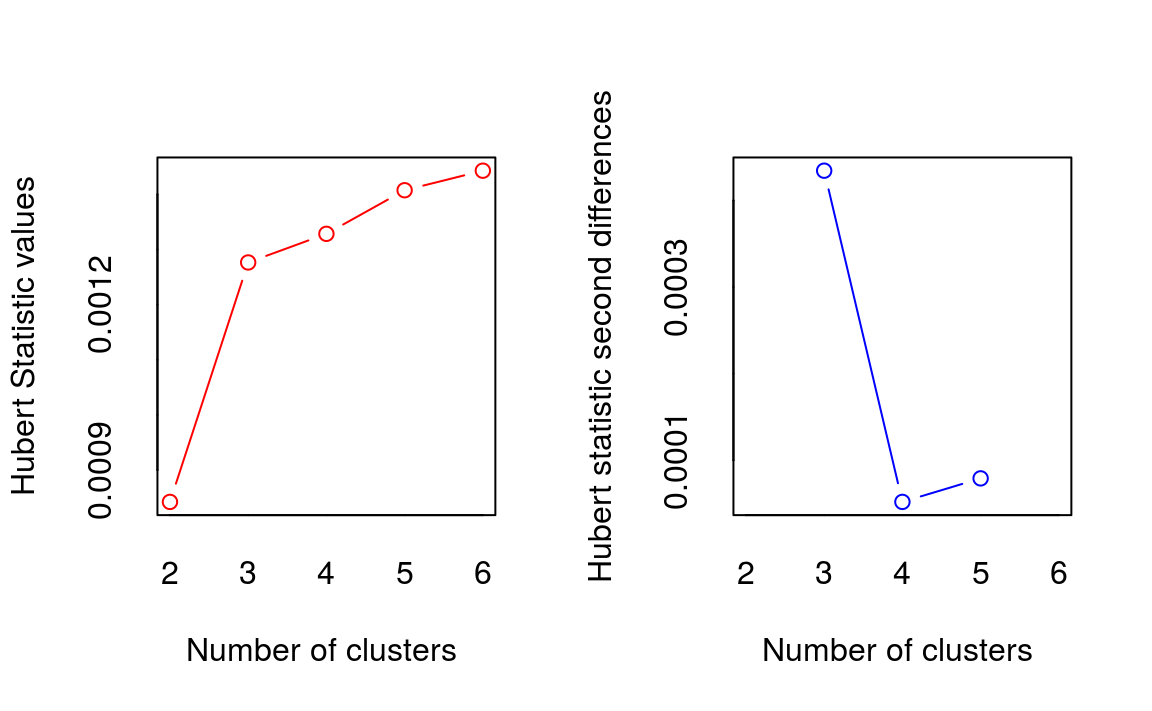
\includegraphics[width=0.5\linewidth]{04-penalized_regression_files/figure-latex/unnamed-chunk-16-1} \end{center}

\(y\)축은 계수의 값이고, \(x\)축은 L1-norm 입니다. 이번에는 람다 값이 바뀜에 따라 계수의 값이 어떻게 바뀌는지 살펴보도록 합니다.

\begin{Shaded}
\begin{Highlighting}[]
\KeywordTok{plot}\NormalTok{(ridge, }\DataTypeTok{xvar =} \StringTok{'lambda'}\NormalTok{, }\DataTypeTok{label =} \OtherTok{TRUE}\NormalTok{)}
\end{Highlighting}
\end{Shaded}

\begin{center}\includegraphics[width=0.5\linewidth]{04-penalized_regression_files/figure-latex/unnamed-chunk-17-1} \end{center}

람다 값이 줄어들수록 벌점이 줄어들고 계수의 절대값이 올라갑니다. 해당 모형을 테스트 셋에 적용해 보도록 합니다.

\begin{Shaded}
\begin{Highlighting}[]
\NormalTok{newx =}\StringTok{ }\KeywordTok{as.matrix}\NormalTok{(test[, }\DecValTok{1}\OperatorTok{:}\DecValTok{8}\NormalTok{])}
\NormalTok{ridge.y =}\StringTok{ }\KeywordTok{predict}\NormalTok{(ridge, }\DataTypeTok{newx =}\NormalTok{ newx, }\DataTypeTok{type =} \StringTok{'response'}\NormalTok{, }\DataTypeTok{s =} \FloatTok{0.1}\NormalTok{)}
\KeywordTok{plot}\NormalTok{(ridge.y, test}\OperatorTok{$}\NormalTok{lpsa, }\DataTypeTok{xlab =} \StringTok{'Predicted'}\NormalTok{, }\DataTypeTok{ylab =} \StringTok{'Actual'}\NormalTok{, }\DataTypeTok{main =} \StringTok{'Ridge Regression'}\NormalTok{)}
\end{Highlighting}
\end{Shaded}

\begin{center}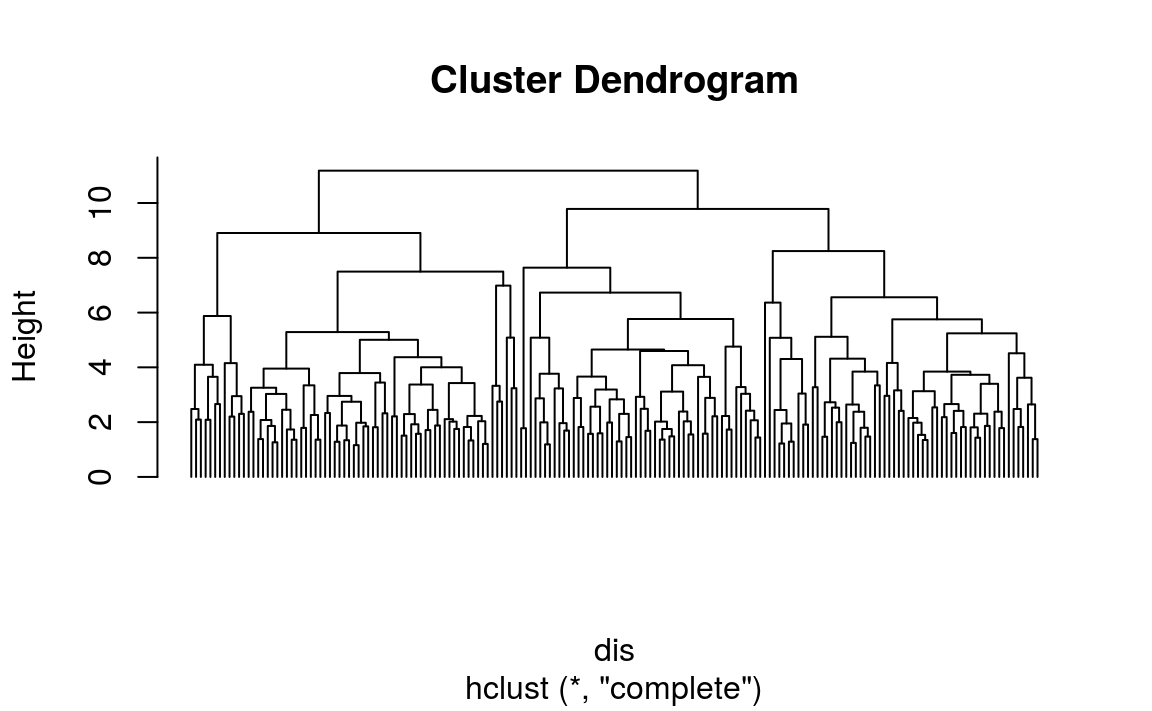
\includegraphics[width=0.5\linewidth]{04-penalized_regression_files/figure-latex/unnamed-chunk-18-1} \end{center}

마지막으로 MSE를 계산하도록 합니다.

\begin{Shaded}
\begin{Highlighting}[]
\NormalTok{ridge.resid =}\StringTok{ }\NormalTok{ridge.y }\OperatorTok{-}\StringTok{ }\NormalTok{test}\OperatorTok{$}\NormalTok{lpsa}
\NormalTok{ridge.mse =}\StringTok{ }\KeywordTok{mean}\NormalTok{(ridge.resid}\OperatorTok{^}\DecValTok{2}\NormalTok{)}
\KeywordTok{print}\NormalTok{(ridge.mse)}
\end{Highlighting}
\end{Shaded}

\begin{verbatim}
## [1] 0.4784
\end{verbatim}

최량 부분 집합의 MSE 보다 약간 줄어들었습니다.

\hypertarget{lasso}{%
\subsubsection{LASSO}\label{lasso}}

\texttt{glmnet()}의 alpha 인자를 1로 변경하면 간단하게 LASSO 분석을 실시할 수 있습니다.

\begin{Shaded}
\begin{Highlighting}[]
\NormalTok{lasso =}\StringTok{ }\KeywordTok{glmnet}\NormalTok{(x, y, }\DataTypeTok{family =} \StringTok{'gaussian'}\NormalTok{, }\DataTypeTok{alpha =} \DecValTok{1}\NormalTok{)}
\end{Highlighting}
\end{Shaded}

\begin{Shaded}
\begin{Highlighting}[]
\KeywordTok{print}\NormalTok{(lasso)}
\end{Highlighting}
\end{Shaded}

\begin{center}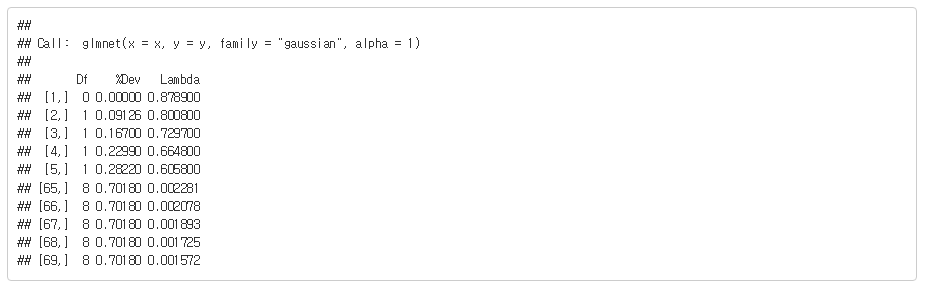
\includegraphics[width=1\linewidth]{images/lasso} \end{center}

모형의 람다 값이 줄어드는 데도 편차가 더 이상 나아지지 않아 69번째에서 멈추게 됩니다.

\begin{Shaded}
\begin{Highlighting}[]
\KeywordTok{plot}\NormalTok{(lasso, }\DataTypeTok{xvar =} \StringTok{'lambda'}\NormalTok{, }\DataTypeTok{label =} \OtherTok{TRUE}\NormalTok{)}
\end{Highlighting}
\end{Shaded}

\begin{center}\includegraphics[width=0.5\linewidth]{04-penalized_regression_files/figure-latex/unnamed-chunk-23-1} \end{center}

해당 모델을 테스트 셋에 적용하고 MSE를 구하도록 합니다.

\begin{Shaded}
\begin{Highlighting}[]
\NormalTok{lasso.y =}\StringTok{ }\KeywordTok{predict}\NormalTok{(lasso, }\DataTypeTok{newx =}\NormalTok{ newx, }\DataTypeTok{type =} \StringTok{'response'}\NormalTok{, }\DataTypeTok{s =} \FloatTok{0.045}\NormalTok{)}
\KeywordTok{plot}\NormalTok{(lasso.y, test}\OperatorTok{$}\NormalTok{lpsa, }\DataTypeTok{xlab =} \StringTok{'Predicted'}\NormalTok{, }\DataTypeTok{ylab =} \StringTok{'Actual'}\NormalTok{, }\DataTypeTok{main =} \StringTok{'LASSO'}\NormalTok{)}

\NormalTok{lasso.resid =}\StringTok{ }\NormalTok{lasso.y }\OperatorTok{-}\StringTok{ }\NormalTok{test}\OperatorTok{$}\NormalTok{lpsa}
\NormalTok{lasso.mse =}\StringTok{ }\KeywordTok{mean}\NormalTok{(lasso.resid }\OperatorTok{^}\DecValTok{2}\NormalTok{)}
\KeywordTok{print}\NormalTok{(lasso.mse)}
\end{Highlighting}
\end{Shaded}

\begin{verbatim}
## [1] 0.4437
\end{verbatim}

\begin{center}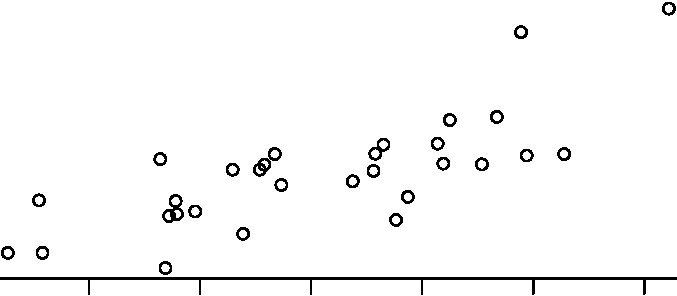
\includegraphics[width=0.5\linewidth]{04-penalized_regression_files/figure-latex/unnamed-chunk-24-1} \end{center}

가장 낮은 MSE를 보입니다. 3가지 모형의 MSE를 비교하면 다음과 같습니다.

\begin{table}[!h]

\caption{\label{tab:unnamed-chunk-25}각 모형의 MSE 비교}
\centering
\begin{tabular}[t]{cc}
\toprule
모형 & MSE\\
\midrule
\rowcolor{gray!6}  최량 부분 집합 & 0.5084\\
Ridge & 0.4784\\
\rowcolor{gray!6}  LASSO & 0.4437\\
\bottomrule
\end{tabular}
\end{table}


\end{document}
